\documentclass[12pt]{article}
\pagestyle{plain}
\topmargin=-0.5in
\textheight=9in
\evensidemargin=-0.35in
\oddsidemargin=-0.35in
\setlength{\textwidth}{7.2in}

\usepackage{graphicx}
\usepackage[shortlabels]{enumitem}
\usepackage{hyperref}
\usepackage{amsthm}
\usepackage{amsmath}
\usepackage{amsfonts}
\usepackage{xcolor}
\usepackage{comment}
\usepackage{bm}
\usepackage{amssymb}
\usepackage{cite}
\usepackage{tikz-cd}
\usetikzlibrary{decorations.pathmorphing}
\usepackage{framed}

\newtheorem{theorem}{Theorem}
\newtheorem{lemma}[theorem]{Lemma}
\newtheorem{proposition}[theorem]{Proposition}
\theoremstyle{definition}
\newtheorem{definition}[theorem]{Definition}
\newtheorem{example}[theorem]{Example}
\newtheorem{remark}[theorem]{Remark}
\newtheorem{exercise}[theorem]{Exercise}

%\numberwithin{theorem}{subsection}

\raggedbottom

\newcommand{\N}{\mathbb{N}}
\newcommand{\Z}{\mathbb{Z}}
\newcommand{\Q}{\mathbb{Q}}
\newcommand{\R}{\mathbb{R}}
\newcommand{\C}{\mathbb{C}}

\newcommand{\sig}{\sigma}
\newcommand{\lam}{\lambda}
\newcommand{\eps}{\varepsilon}

\newcommand{\lp}{\left(}
\newcommand{\rp}{\right)}
\newcommand{\lb}{\left\{}
\newcommand{\rb}{\right\}}
\newcommand{\lab}{\left|}
\newcommand{\rab}{\right|}
\newcommand{\la}{\left\langle}
\newcommand{\ra}{\right\rangle}

\newcommand{\tbf}{\textbf}
\newcommand{\noi}{\noindent}
\newcommand{\incomplete}{\textcolor{red}{INCOMPLETE}}

\newcommand{\inv}{^{-1}}
\newcommand{\sm}{\setminus}
\newcommand{\wt}{\widetilde}
\newcommand{\wh}{\widehat}
\newcommand{\ov}{\overline}

\newcommand{\iso}{\cong}

\newcommand{\frakg}{\mathfrak{g}}
\newcommand{\fraksl}{\mathfrak{sl}}
\newcommand{\frakso}{\mathfrak{so}}
\newcommand{\fraksu}{\mathfrak{su}}

\DeclareMathOperator{\Hom}{Hom}
\DeclareMathOperator{\characteristic}{char}

\DeclareMathOperator{\M}{M}
\DeclareMathOperator{\Mat}{Mat}
\DeclareMathOperator{\EL}{EL}
\DeclareMathOperator{\SL}{SL}
\DeclareMathOperator{\GL}{GL}
\DeclareMathOperator{\SU}{SU}
\DeclareMathOperator{\OO}{O}
\DeclareMathOperator{\SO}{SO}
\DeclareMathOperator{\diag}{diag}
\DeclareMathOperator{\Id}{Id}
\DeclareMathOperator{\Tr}{Tr}
\DeclareMathOperator{\tr}{tr}
\DeclareMathOperator{\Aut}{Aut}
\DeclareMathOperator{\rad}{rad}

\title{Pinning-Sympy: Theoretical Underpinnings}
\author{Joshua Ruiter}

\begin{document}
\maketitle
\tableofcontents

\newpage

\section{Big picture}

Algebraic groups have two structures. An abstract homomorphism between algebraic groups is a map that preserves one of the structures, but not necessarily the other. We want to prove that abstract homomorphisms are more rigid than they initially appear, by proving that they ``kind of" preserve the other structure.

\subsection{What is an algebraic group?}

For the purposes of these notes, an algebraic group is a set which is both an algebraic variety (over a base field $k$), and a group. The algebraic variety structure is a ``geometric" thing. A variety is a set of solutions to some polynomial equations. Polynomial equations are geometric in the sense that the set of solutions is something we can graph. 

In this project, we are more focused on the ``group" aspect of algebraic groups. The group side is something we can study from an abstract algebra and group theory perspective. We can analyze subgroups, conjugation, group homomorphisms, kernels, etc. 

Group homomorphisms are an effective tool for extracting information about groups. The analogous tool for algebraic varieties is a regular map, which is roughly speaking something that behaves like a polynomial function. Usually, people studying algebraic groups study morphisms of algebraic groups, which are group homomorphisms that are also regular maps. However, you can also just look at ``abstract" homomorphisms between algebraic groups, which is to say, just group homomorphisms that ignore the geometric structure.

\subsection{What is rigidity?}

To illustrate the idea of rigidity, we go on an aside about continuity and differentiability. In general, a continuous function $f:\R \to \R$ is not infinitely differentiable, and may even fail to be differentiable a single time. (By ``differentiable,'' we mean ``differentiable everywhere.") A continuous function may have corners ($y=|x|$) or cusps ($y=x^{2/3}$). On the other hand, every differentiable function is continuous. In the world of continuous functions, at one extreme are the ``very differentiable" and ``very continuous" polynomial functions. At the other end, there are continuous functions which are not differentiable anywhere, such as the Weierstrass function\footnote{\url{https://en.wikipedia.org/wiki/Weierstrass_function}}. In the diagram below, we depict a ``rigidity spectrum" for continuous functions, with rigidity increasing to the right.

\begin{center}
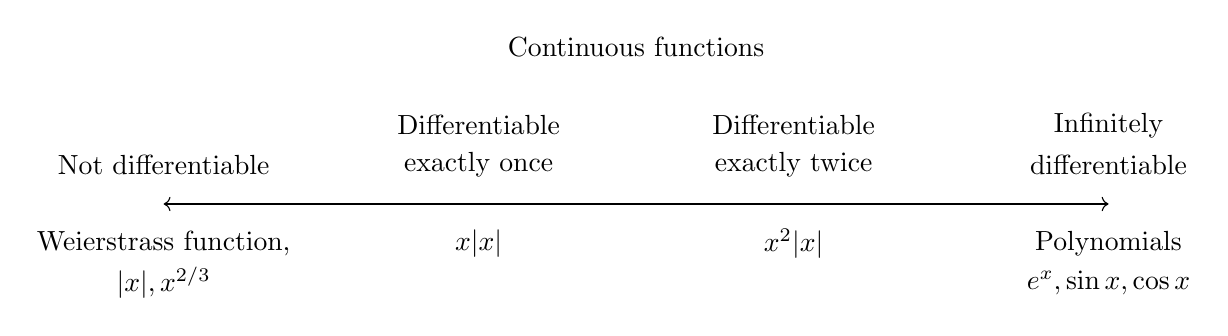
\begin{tikzpicture}
	\node[] at (0,2) {Continuous functions};
	\draw[<->](-6,0) -- (6,0);
	
	\node[] at (-6,0.5) {Not differentiable};
	\node[] at(-6,-0.5) {Weierstrass function,};
	\node[] at (-6,-1) {$|x|, x^{2/3}$};

	\node[] at (-2,1) {Differentiable};
	\node[] at (-2, 0.5) {exactly once};
	\node[] at (-2,-0.5) {$x|x|$};

	\node[] at (2, 1) {Differentiable};
	\node[] at (2, 0.5) {exactly twice};
	\node[] at (2,-0.5) {$x^2|x|$};

	\node[] at (6,1) {Infinitely};
	\node[] at (6,0.5) {differentiable};
	\node[] at (6,-0.5) {Polynomials};
	\node[] at (6,-1) {$e^x, \sin x, \cos x$};
\end{tikzpicture}
\end{center}
The main issue with the graphic above is that actually, differentiable functions are extremely rare among all continuous functions. A better visualization would have 99\% of the spectrum devoted to functions like the Weierstrass function which are continuous but differentiable at no points or just a finite set of points.

In parallel to the discussion above, morphisms of algebraic groups are much more rigid than abstract homomorphisms. So we do not, in general, expect an abstract homomorphism to be regular. However, sometimes we can prove that an abstract homomorphism is ``almost" regular, in a particular sense. These are called ``rigidity theorems."

We want to prove rigidity theorems of the following form: for a particular fixed algebraic group $G(k)$, any abstract homomorphism $\rho:G(k) \to \GL_m(K)$ must be ``almost regular'' ($K$ is some field extension of $k$). In this context, ``almost regular" means a factorization of $\rho$, a way of writing $\rho$ as a composition of two maps, where one of those is regular. The usual goal is to factor $\rho$ into the form $\rho = \sig \circ F$ where $\sig$ is regular.
\begin{center}
	\begin{tikzcd}
		G(k) \arrow[rightsquigarrow]{dr}[swap]{F} \arrow[rightsquigarrow]{rr}{\rho} && \GL_m(K) \\
		& G(A) \arrow{ur}[swap]{\sig}
	\end{tikzcd}
\end{center}
Here $A$ is some algebra. To emphasize the rigidity of $\sig$, the diagram above uses squiggly arrows for abstract group homomorphisms, and a straight arrow for the more rigid regular group homomorphism. Philosophically speaking, we think of $\sig$ as the ``regular part" of $\rho$.

\subsection{What is a pinning?}

Algebraic groups have a lot of structure. We can ``pin" them to understand and see the structure better. The word ``pinning" here comes from the metaphor of pinning the wings of a butterfly specimen, as you might see in a museum. A pinning of an algebraic group $G(k)$ is a collection of functions
\[
	X_\alpha:V_\alpha(k) \to G(k)
\]
where $\alpha$ ranges over the set of ``roots'' $\Phi$ of $G$, and $V_\alpha(k)$ is just a vector space over $k$ (often the dimension of $V_\alpha(k)$ is just one, so in that case $V_\alpha(k)$ is essentially just $k$ with the group operation of addition). These pinning maps $X_\alpha$ should satisfy a variety of properties.
\begin{enumerate}[(P1)]
	\item They are \textit{usually} group homomorphisms, meaning that
	\[
		X_\alpha(v) \cdot X_\alpha(w) = X_\alpha(v+w)
	\]
	for all $v,w \in V_\alpha(k)$. More generally, this equation might fail and there will need to be an additional factor on one side to account for this defect.
	\[
		X_\alpha(v) \cdot X_\alpha(w) = X_{\alpha}(v+w) \cdot \Big( \text{correction term} \Big)
	\]
	\item The group $G(k)$ is generated by the images $X_\alpha \big( v \big)$, where $\alpha$ ranges over $\Phi$ and $v$ ranges over $V_\alpha(k)$.
	\item $G(k)$ contains a subgroup $T(k)$ called a ``maximal $k$-split torus" and for any $t \in T(k)$, conjugating $X_\alpha(v)$ by $t$ corresponds to scalar multiplication of the input vector $v$ by a scalar called $\alpha(t)$.
	\[
		t \cdot X_\alpha(v) \cdot t \inv = X_\alpha \Big( \alpha(t) \cdot v \Big)
	\]
	\item There is a ``Weyl group" $W$ and for any root $\alpha \in \Phi$, there is a corresponding Weyl group element $w_\alpha \in G(k)$. Also, for any root $\beta \in \Phi$, conjugating $X_\beta(v)$ by $w_\alpha$ corresponds to changing the root $\beta$ by some kind of reflection process to get a new root $\sig_\alpha(\beta)$, and doing some invertible linear transformation $\phi$ to $v$.
	\[
		w_\alpha \cdot X_\beta(v) \cdot w_\alpha \inv = X_{\sig_\alpha(\beta)} \Big( \varphi(v) \Big)
	\]
	Ideally, $\varphi$ is not very complicated, something like $\phi(v) = -v$, but sometimes it might be something like: thinking of $v$ as a vector with a 3 or 4 components, $\varphi(v)$ permutes these components and adds some negative signs to some of them.
	\item Given two roots $\alpha$ and $\beta$ with $\alpha+\beta \neq 0$, the commutator
	\[
		\Big[ X_\alpha(v), X_\beta(w) \Big] = \prod_{?} X_\gamma\Big( N(u,v) \Big)
	\]
	is some product of other pinning map outputs $X_{\gamma}$ and the inputs of those are determined by some function $N$ (a polynomial function of $u$ and $v$). This product is determined by the root system $\Phi$. Often $N(u,v)$ is something like
\[
	N(u,v) = \pm uv
\]
or
\[
	N(u,v) = c_1 u_1 v_1 + c_2 u_2 v_2 + \cdots + c_n u_n v_n
\]
where $u = (u_1, \ldots, u_n)$ and $v = (v_1, \ldots, v_n)$ and the $c_i$ are coefficients coming from the definition of the group $G$.
\end{enumerate}

\noi Next up are some exercises to get a better hands-on understanding of some aspects of the pinning definition. For all of the exercises below, fix a field $k$.

\begin{exercise}
Let $G$ be a group of matrices, and let $X:k \to G$ be a group homomorphism from $(k, +)$ to $G$. That is,
\[
	X(u + v) = X(u) \cdot X(v)
\]
where $+$ on the left means addition in $k$, and $\cdot$ on the right means matrix multplication. Show that $X(0)$ is the identity matrix. (Combined with property (P1), what does this say about pinning maps?)
\end{exercise}

\begin{exercise}
Show that any matrix of the form
\[
	\begin{pmatrix}
		1 & a & b \\
		& 1 & c\\
		&& 1
	\end{pmatrix}
\]
with $a,b,c \in k$ can be written as a product of matrices of the form
\[
	\begin{pmatrix}
		1 & u &  \\
		& 1 & \\
		&& 1
	\end{pmatrix}
	\qquad
	\begin{pmatrix}
		1 & & v  \\
		& 1 & \\
		&& 1
	\end{pmatrix}
	\qquad
	\begin{pmatrix}
		1 & &  \\
		& 1 & w \\
		&& 1
	\end{pmatrix}
\]
Be careful: It's not just as simple as the product
\[
	\begin{pmatrix}
		1 & a &  \\
		& 1 & \\
		&& 1
	\end{pmatrix}
	\begin{pmatrix}
		1 & & b  \\
		& 1 & \\
		&& 1
	\end{pmatrix}
	\begin{pmatrix}
		1 & &  \\
		& 1 & c \\
		&& 1
	\end{pmatrix}
\]
This exercise is illustrating how $\SL_3(k)$ is generated by the images of its pinning maps, a la property (P2). We will study this pinning in detail in section \ref{special linear}. The set of all matrices of this form also has a name: the group of \tbf{unipotent} matrices.
\end{exercise}

\begin{exercise}
Let $t_1, t_2, t_3 \in k^\times$ be nonzero elements of $k$. Let $t = \diag(t_1, t_2, t_3)$ be an arbitrary $3 \times 3$ diagonal matrix with entries in $k^\times$. Let
\[
	X = X_{\alpha_{12}}(u) = 
	\begin{pmatrix}
		1 & u \\
		& 1 \\
		&& 1
	\end{pmatrix}
\]
Verify by direct calculation that
\[
	t \cdot X \cdot t \inv = X_{\alpha_{12}}(t_1 t_2 \inv u) = 
	\begin{pmatrix}
		1 & t_1 t_2 \inv u \\
		& 1 \\
		&& 1
	\end{pmatrix}
\]
(This is just one example of (P3) for $\SL_3(k)$.)
\end{exercise}

\begin{exercise}
Let $X$ and $Y$ be the matrices below.
\[
	X = X_{\alpha_{12}}(u) = 
	\begin{pmatrix}
		1 & u \\
		& 1 \\
		&& 1
	\end{pmatrix}
	\qquad
	Y = X_{\alpha_{23}}(v) = 
	\begin{pmatrix}
		1 & \\
		& 1 & v \\
		&& 1
	\end{pmatrix}
\]
Verify that the commutator $[X,Y]$ has the form
\[
	X_{\alpha_{13}}( N(u,v) ) = 
	\begin{pmatrix}
		1 & & N(u,v) \\
		& 1 & \\
		&& 1
	\end{pmatrix}
\]
and determine a formula for $N(u,v)$, thinking of $N$ as a function $N:k \times k \to k$. (This is an example of (P5) for $\SL_3(k)$.)
\end{exercise}

\newpage
\section{Special linear groups}
\label{special linear}

Fix a field $k$. Whenever convenient, we can assume that the characteristic of $k$ is zero. This assumption is mostly not necessary, but it simplifies some things. The group of units of $k$ is denoted $k^\times$ (in other words, $k^\times$ is the set of nonzero elements in $k$).

\begin{definition}
Fix a field $k$ and a positive integer $n$. $\M_n(k)$ is the set of $n \times n$ matrices with entries in $k$. For $x \in \M_n(k)$, the \tbf{determinant} of $x$ is an element of $k$. For $2 \times 2$ matrices, the usual formula applies.
\[
	\det
	\begin{pmatrix}
		a & b \\
		c & d
	\end{pmatrix}
	= ad - bc
\]
For $3 \times 3$ matrices, we can use the $2 \times 2$ formula and a cofactor expansion to calculate the determinant.
\[
	\det
	\begin{pmatrix}
		a & b & c \\
		d & e & f \\
		g & h & i
	\end{pmatrix}
	= a \cdot \det
	\begin{pmatrix}
		e & f \\
		h & i
	\end{pmatrix}
	-
	b \cdot \det
	\begin{pmatrix}
		d & f \\
		g & i
	\end{pmatrix}
	+ c  \cdot \det
	\begin{pmatrix}
		d & e \\
		g & h
	\end{pmatrix}
\]
This process generalizes to larger $n \times n$ matrices. To calculate the determinant, we expand along the top row. We should not actually have to do this by hand at any point. The point being made here is just that the determinant of an $n \times n$ matrix is defined over any field $k$, because calculating a determinant only involves addition and multiplication operations in the field $k$.
\end{definition}

\begin{definition}
Fix a positive integer $n$. The \tbf{special linear group} with coefficients in $k$ is the group of $n \times n$ matrices with determinant 1.
\[
	\SL_n(k) = \lb X \in \M_n(k) : \det X = 1 \rb
\]
$\SL_n(k)$ is an algebraic group under matrix multiplication. The condition $\det(X) = 1$ may not initially appear to be a polynomial equation, but if you expand out the determinant, it is just a big polynomial in terms of the coefficients of the matrix $X$.
\end{definition}

\subsection{Torus subgroup and character group}

\begin{definition}
The \tbf{diagonal subgroup} or \tbf{torus subgroup} in $\SL_n(k)$ is the subgroup of diagonal matrices. We will call it $T(k)$.
\[
	T(k) =
	\lb
	\begin{pmatrix}
		t_1 \\
		& t_2 \\
		&& \ddots \\
		&&& t_n
	\end{pmatrix}
	: t_i \in k^\times, \det t = t_1 t_2 \cdots t_n = 1
	\rb
\]
Notice that the equation $t_1 t_2 \cdots t_n = 1$ means that none of the entries $t_i$ can be zero for an element of $T(k)$. For an element of $T(k)$, the inverse is the matrix whose diagonal entries are the term-by-term inverses.
\[
	\begin{pmatrix}
		t_1 \\
		&& \ddots \\
		&&& t_n
	\end{pmatrix}
	\inv
	=
	\begin{pmatrix}
		t_1 \inv \\
		&& \ddots \\
		&&& t_n \inv
	\end{pmatrix}
\]
\end{definition}

\begin{definition}
Let $T(k)$ be the diagonal subgroup of $\SL_n(k)$ as above. For $i=1, \ldots, n$, define a map $\alpha_i:T(k) \to k^\times$ by
\[
	\alpha_i
	\begin{pmatrix}
		t_1 \\
		& t_2 \\
		&& \ddots \\
		&&& t_n
	\end{pmatrix}
	= t_i
\]
Since the determinant of an element of $T(k)$ is one, none of the individual diagonal entries $t_i$ can be zero, so $t_i \in k^\times$. More importantly, $\alpha_i$ is a group homomorphism, meaning $\alpha_i(ts) = \alpha_i(t) \alpha_i(s)$ for any $s,t \in T(k)$.
\end{definition}

\begin{definition}
The \tbf{character group} of $T(k)$ is the set of group homomorphisms from $T(k)$ to $k^\times$. It is called $X(T(k))$ or just $X(T)$.
\[
	X(T) = \Hom(T(k), k^\times) = \lb \alpha:T(k) \to k^\times \mid \alpha \text{ is a group homomorphism} \rb
\]
Group homomorphisms $T(k) \to k^\times$ are called \tbf{characters} (of $T$). The \tbf{sum} of two characters $\alpha$ and $\beta$ is defined to be
\[
	\alpha+\beta:T(k) \to k^\times \qquad (\alpha+\beta)(t) = \alpha(t)  \beta(t)
\]
where the multiplication on the right side is just multiplication in $k$. The set of characters $X(T)$ is an abelian group under this character sum operation (you checked this on the application last fall). In particular, the identity of $X(T)$ is the constant function
\[
	0_{X(T)}:T(k) \to k^\times \qquad t \mapsto 1
\]
We call this function the \tbf{zero character}, and usually just denote it by $0$. (You can check that $\alpha + 0_{X(T)} = \alpha$ for any $\alpha \in X(T)$.)
\end{definition}

\begin{definition}
Let $T(k)$ and $\alpha_i$ be as above. For $1 \le i,j \le n$ and $i \neq j$, define $\alpha_{ij} = \alpha_i - \alpha_j$. In other words, $\alpha_{ij}$ is a group homomorphism $T(k) \to k^\times$ (that is, $\alpha_{ij}$ is a character of $T$), and it is described by
\begin{align*}
	\alpha_{ij}(t) = (\alpha_i - \alpha_j)(t) = \alpha_i(t) \alpha_j(t) \inv = 
	\alpha_{ij}
	\begin{pmatrix}
		t_1 \\
		& \ddots \\
		&& t_n
	\end{pmatrix} = t_i t_j \inv
\end{align*}
\end{definition}

\begin{remark}
In $T(k)$, we have the equation $\det(t) = 1$. Since the determinant of a diagonal matrix is the product of the diagonal entries, we get the equation
\[
	1 = \det(t) = t_1 \cdots t_n = \alpha_1(t) \cdots \alpha_n(t)
\]
That is,
\[
	\alpha_1(t) \cdots \alpha_n(t) = 1 = 0_{X(T)}(t)
\]
where $0_{X(T)} \in X(T)$ is the zero character. In other words, the sum
\[
	\alpha_1 + \cdots + \alpha_n \in X(T)
\]
is the zero character. Translating this into an equation in $X(T)$, we get the following.
\[
	\alpha_1 + \cdots + \alpha_n = 0_{X(T)} = 0
\]
We emphasize: this is not an equation in $k$, it is an equation in the abelian group $X(T)$.
\end{remark}

\begin{definition}
For $n \ge 1$, define $\Z^n = \Z \oplus \cdots \oplus \Z$ ($n$ copies of $\Z$).
\end{definition}

\begin{lemma}
Let $\Z \vec 1$ be the set of integer multiples of the vector $\vec 1 = (1, \ldots, 1)$.
\[
	\Z \vec 1 = \lb m(1, \ldots, 1) = (m, \ldots, m) : m \in \Z \rb
\]
Then $X(T) \iso \Z^n / \Z \vec 1$ (isomorphism of abelian groups).
\end{lemma}
\begin{proof}
Let $e_i \in \Z^{n}$ be the $n$-tuple $(0, \ldots, 0, 1, 0, \ldots, 0)$ which is all zeros except for a one in the $i$th position. Then consider the map
\[
	\phi:\Z^n \to X(T) \qquad \phi \lp \sum_{i=1}^n m_i e_i \rp = \sum_{i=1}^n m_i \alpha_i
\]
where the $m_i$ are integers. Then $\phi$ is a group homomorphism, $\ker \phi = \Z \vec 1$, and $\phi$ is onto, so by the first isomorphism theorem, $\Z^n / \ker \phi = \Z^n / \Z \vec 1 \iso X(T)$.
\end{proof}

\noi The following elements correspond under the above isomorphism.
\begin{align*}
	e_i &\longleftrightarrow \alpha_i \\
	e_i - e_j &\longleftrightarrow \alpha_{ij} = \alpha_i - \alpha_j \\
	(1, -1, 0, 0, \ldots, 0) &\longleftrightarrow \alpha_{12} = \alpha_1 - \alpha_2 \\
	(0, 1, -1, 0, \ldots, 0) &\longleftrightarrow \alpha_{23} = \alpha_2 - \alpha_3 \\
	(0, 0, 1, -1, \ldots, 0) &\longleftrightarrow \alpha_{34} = \alpha_3 - \alpha_4
\end{align*}
This is somewhat misleading -- more literally, on the left side of this correspondence I mean that the coset $\ov e_i = e_i + \Z \vec 1$ corresponds to the character $\alpha_i$, and so on. This becomes apparent when we consider the corresponding elements
\[
	\vec 1 = (1, \ldots, 1) \longleftrightarrow \alpha_1 + \cdots + \alpha_n
\]
because $\alpha_1 + \cdots + \alpha_n = 0$ in $X(T)$, but $\vec 1$ is not the zero element in $\Z^n$. However, $\vec 1$ does represent the zero coset in the quotient $\Z^n / \Z \vec 1$; that is, $\vec 1 + \Z \vec 1 = \Z \vec 1 = 0$ in $\Z^n / \Z \vec 1$.

\subsection{Pinning the special linear group}

Let $k$ be a field of characteristic zero, and consider the special linear group $\SL_n(k)$.

\begin{definition}
Fix $i, j$ with $1 \le i, j \le n$ and $i \neq j$. For $x \in k$, let $E_{ij}(x)$ be the matrix with $x$ in the $ij$ entry and 0 elsewhere. Let $e_{ij}(x) = I + E_{ij}(x)$ be the matrix with $x$ in the $ij$ entry, 1's on the diagonal, and 0 elsewhere. For example, in $\SL_2(k)$ we have
\[
	E_{12}(x) =
	\begin{pmatrix}
		0 & x \\
		0 & 0
	\end{pmatrix}
	\qquad
	e_{12}(x) =
	\begin{pmatrix}
		1 & x \\
		0 & 1
	\end{pmatrix}
\]
The determinant of $e_{ij}(x)$ is one, so $e_{ij}(x) \in \SL_n(k)$. Now, consider $e_{ij}$ as a group homomorphism from $k$ (viewed as an abelian group under addition) to $\SL_n(k)$.
\[
	e_{ij}:k \to \SL_n(k) \qquad x \mapsto e_{ij}(x)
\]
This being a group homomorphism means that
\[
	e_{ij}(x+y) = e_{ij}(x) \cdot e_{ij}(y)
\]
Since $e_{ij}$ is a homomorphism, it must take the identity to the identity.
\[
	e_{ij}(0) = I =1 \in \SL_n(k)
\]
Also notice that $\ker \lp e_{ij} \rp = \lb 0 \rb$, so $e_{ij}$ is injective. 
\end{definition}

\begin{definition}
Instead of $e_{ij}$, we will use the notation $X_{\alpha_{ij}}$ for the same thing. That is, $X_{\alpha_{ij}}(u) = e_{ij}(u)$ for $u \in k$.
\end{definition}

\begin{remark}
It is useful to remember that $X_{\alpha_{ij}}(u) \inv = X_{\alpha_{ij}}(-u)$. This is a consequence of the fact that $X_{\alpha_{ij}}$ is a group homomorphism.
\end{remark}

\begin{definition}
The \tbf{root system} of $\SL_n(k)$ is the set of characters $\alpha_{ij}$ for $i \neq j$. We denote it by $\Phi(\SL_n(k), T(k))$ or $\Phi(\SL_n, T)$ or just $\Phi$.
\[
	\Phi = \lb \alpha_{ij} : 1 \le i, j \le n, i \neq j \rb
\]
Elements of $\Phi$ are called \tbf{roots}. It is important not to forget that elements of $\Phi$ are characters, i.e. functions from $T(k)$ to $k^\times$. Specifically, $\alpha_{ij}$ is the function
\[
	\alpha_{ij}:T(k) \to k^\times \qquad \alpha_{ij}(t) = \alpha_i(t) \alpha_j(t) \inv = t_i t_j \inv
\]
where $t = \diag(t_1, \ldots, t_n)$.
\end{definition}


\subsubsection{Conjugation by torus}

$T(k)$ acts on $\SL_n(k)$ by conjugation. That is, there is a group action 
\[
	T(k) \times \SL_n(k) \to \SL_n(k) \qquad t * x = txt \inv
\]

\begin{exercise}
Verify that this is a group action, by showing that
\begin{itemize}
	\item For any $t \in T(k)$ and $x \in \SL_n(k)$, the conjugation $t*x = txt \inv$ is in $\SL_n(k)$.
	\item If $I$ is the identity matrix and $x \in \SL_n(k)$, then $I * x = Ix I \inv = x$.
	\item For any two elements $s, t \in T(k)$, we have $(ts) * x  = t * (s * x)$. 
\end{itemize}
\end{exercise}


\begin{lemma}
Let $1 \le i,j \le n$ and $i \neq j$. Let $t \in T(k)$ be a diagonal matrix, and let $u \in k$. Then
\[
	t * X_{\alpha_{ij}}(u) = t \cdot X_{\alpha_{ij}(u)} \cdot t \inv = X_{\alpha_{ij}} \Big( \alpha_{ij}(t) u \Big)
\]
In other words, for $\alpha \in \Phi(\SL_n(k), T(k))$, we have
\[
	t * X_\alpha(u) = t \cdot X_\alpha(u) \cdot t \inv = X_\alpha \Big( \alpha(t) u \Big)
\]
\end{lemma}

\begin{exercise}
In the group $\SL_2(k)$, confirm by direct matrix calculation that for any $t = \diag(t_1, t_2)$ and $u \in k$, that we have
\[
	t \cdot X_{\alpha_{12}}(u) \cdot t \inv = X_{\alpha_{12}} \Big( \alpha_{12}(t) u \Big) = X_{\alpha_{12}} ( t_1 t_2 \inv u )
\]
That is,
\[
	\begin{pmatrix}
		t_1 \\
		& t_2
	\end{pmatrix}
	\begin{pmatrix}
		1 & u \\
		& 1
	\end{pmatrix}
	\begin{pmatrix}
		t_1 \\
		& t_2
	\end{pmatrix} \inv
	=
	\begin{pmatrix}
		1 & t_1 t_2 \inv u  \\
		& 1
	\end{pmatrix}
\]
Then convince yourself that nothing really changes when you do the ``same" calculation in $\SL_n(k)$, replacing $t$ with $\diag(t_1, t_2, \ldots, t_n)$.
\end{exercise}


\subsubsection{Conjugation by Weyl group}

\begin{definition}
Let $\alpha \in \Phi(\SL_n(k), T(k))$ be a root, so $\alpha = \alpha_{ij}$ for some $i \neq j$. Let $u \in k$, and assume $u \neq 0$. Then define
\[
	w_\alpha(u) = X_\alpha(u) \cdot X_{-\alpha}( -u \inv) \cdot X_\alpha(u)
\]
Here, $-\alpha$ means the negative of $\alpha$ in the abelian group $X(T)$. Concretely, if $\alpha = \alpha_{ij} = \alpha_i - \alpha_j$, then $- \alpha = \alpha_{ji} = \alpha_j - \alpha_i$. The elements $w_\alpha(u)$ are called \tbf{Weyl group elements}. (There is a larger ``Weyl group" including the $w_\alpha(u)$, but we omit the details for now.)
\end{definition}

\begin{example}
In the group $\SL_3(k)$, with $\alpha = \alpha_{12} = \alpha_1 - \alpha_2$, where $X_\alpha(u) = e_{12}(u)$, that we get
\[
	w_\alpha(1) = w_{\alpha_{12}}(1) =
	\begin{pmatrix}
		& 1 \\
		-1 \\
		&& 1
	\end{pmatrix}
\]
\end{example}

\begin{exercise}
Work out $w_{\alpha_{12}}(u)$ in more generality (still in $\SL_3(k)$), by doing concrete matrix multiplication with $e_{12}(u)$ matrices.
\end{exercise}

\begin{definition}
A \tbf{monomial matrix} is a matrix with exactly one nonzero entry in each row and each column. A \tbf{permutation matrix} is a monomial matrix where all nonzero entries are 1. A \tbf{signed permutation matrix} is a monomial matrix where all nonzero entries are 1 or $-1$.
\end{definition}

\begin{remark}
In general, for $\alpha \in \Phi(\SL_n(k), T(k))$, the Weyl group elements $w_\alpha(u)$ are monomial matrices, and $w_\alpha(1)$ is a signed permutation matrix.
\end{remark}

\begin{exercise}
Show that for $\alpha \in \Phi(\SL_n(k), T(k))$ and $u \in k^\times$, $w_\alpha(u) \inv = w_\alpha(-u)$.
\end{exercise}

\begin{definition}
Consider the space $\R^n$, and denote the dot product of two vectors $v, w \in \R^n$ by $(v, w)$. Given $v \in \R^n$, the \tbf{hyperplane perpendicular to $v$} is the set of all vectors perpendicular to $v$.
\[
	P_v = \lb w \in \R^n : (v,w) = 0 \rb
\]
The \tbf{reflection across $P_v$} is the (linear) map
\[
	\sig_v:\R^n \to \R^n \qquad \sig_v(w) = w - \frac{2 (v,w)}{(v,v)} v
\]
Geometrically, this is actually a mirror reflection across $P_v$. Now consider $\Phi = \Phi(\SL_n(k), T(k))$. Identify $\Phi$ with a subset of $\R^n$ by identifying $\alpha_i$ with the standard basis vector $e_i = (0,  \ldots, 0, 1, 0, \ldots, 0)$ with the 1 in the $i$th position. Then $\alpha_{ij} = \alpha_i - \alpha_j$ is identified with
\[
	\alpha_{ij} \leftrightarrow (0, \ldots, 0, 1, 0, \ldots, 0, -1, 0, \ldots ,0)
\]
with the $1$ in the $i$th position and $-1$ in the $j$th position. Under this identification, the dot product operation on $\R^n$ becomes
\[
	(\alpha_i, \alpha_j) = \delta_{ij} =
	\begin{cases}
		1 & i = j \\
		0 & i \neq j
	\end{cases}
\]
and then
\begin{align*}
	(\alpha_{ij}, \alpha_{k\ell}) &= (\alpha_i - \alpha_j, \alpha_k - \alpha_\ell) \\
	&= (\alpha_i, \alpha_k) - (\alpha_i, \alpha_{\ell}) - (\alpha_j, \alpha_k) + (\alpha_{j}, \alpha_\ell) \\
	&= \delta_{ik} - \delta_{i\ell} - \delta_{jk} + \delta_{j\ell} \\
	&\in \lb -2, -1, 0, 1, 2 \rb
\end{align*}
Now, for $\alpha \in \Phi$, consider $\alpha$ as an element of $\R^n$ under the identification above. Then we have a hyperplane $P_\alpha$ of vectors perpendicular to $\alpha$, and we can again use the reflection $\sig_\alpha$ across $P_\alpha$.
\[
	\sig_\alpha:\R^n \to \R^n \qquad \sig_\alpha(w) = w - \frac{2 (\alpha,w)}{(\alpha,\alpha)} \alpha
\]
\end{definition}

\begin{lemma}
Let $\alpha \in \Phi = \Phi(\SL_n(k), T(k))$, and let $\sig_\alpha$ be the reflection above. If $\beta \in \Phi$, then $\sig_\alpha(\beta) \in \Phi$. In other words, $\sig_\alpha$ can be thought of as a map $\Phi \to \Phi$.
\[
	\sig_\alpha:\Phi \to \Phi \qquad \sig_\alpha(\beta) = \beta - \frac{2 (\alpha,\beta)}{(\alpha,\alpha)} \alpha
\]
\end{lemma}

\begin{example}
When $n= 3$, we have
\[
	\Phi = \Phi(\SL_n, T) = \lb \alpha_{12}, \alpha_{21}, \alpha_{13}, \alpha_{31}, \alpha_{23}, \alpha_{32} \rb
\]
We identify $\Phi$ with a subset of $\R^3$, the set of vectors
\[
	\wt \Phi = \lb (1,-1,0), (-1,1,0), (1,0,-1), (-1,0,1), (0,1,-1), (0,-1,1) \rb
\]
These vectors are all perpendicular to the vector $(1,1,1)$. In other words, $\wt \Phi$ sits inside a 2D plane, so we can visualize $\wt \Phi$ in two dimensions. When we do, it looks like six vectors pointing at the six vertices of a regular hexagon. 

Try to convince yourself that if you take any two of those vectors $v$ and $w$, take $P_v$ to be the line perpendicular to $v$, and reflect $w$ across $P_v$, then that reflection $\sig_v(w)$ is another one of the six vectors in $\Phi$.
\end{example}

\begin{proposition}
Let $\alpha, \beta \in \Phi(\SL_n(k), T(k))$ be roots. Then
\[
	w_\alpha(1) \cdot X_\beta(u) \cdot w_\alpha(1) \inv = X_{\sig_\alpha (\beta)} \lp \pm u \rp
\]
\end{proposition}

\subsubsection{Commutator formula}

\begin{definition}
Let $G$ be any group, and let $x,y \in G$. The \tbf{commutator} of $x$ and $y$ is
\[
	[x,y] = x y x \inv y \inv
\]
\end{definition}

\begin{exercise}
Show that $x$ and $y$ commute (i.e. $xy= yx$) if and only if $[x,y] = 1$ (here $1$ is the identity element of the group $G$).
\end{exercise}

\begin{exercise}
Let $u, v \in k$. In the group $\SL_n(k)$, compute the commutator
\[
	\Big[ X_{\alpha_{12}}(u), X_{\alpha_{23}}(v) \Big]
\]
\end{exercise}

\begin{proposition}
Let $\Phi = \Phi(\SL_n(k), T(k))$, and let $\alpha, \beta \in \Phi$ so that $\alpha \neq \pm \beta$. Let $u,v \in k$. Then
\[
	\Big[ X_\alpha(u), X_\beta(v) \Big] =
	\begin{cases}
		I & \alpha+\beta \not \in \Phi \\
		X_{\alpha+\beta}( \pm uv) & \alpha+\beta \in \Phi \\
	\end{cases}
\]
That is, $X_\alpha(u)$ and $X_\beta(v)$ commute if and only if $\alpha+\beta \not \in \Phi$ (or if $uv = 0$). 
\end{proposition}

\begin{remark}
The signs in the previous proposition can be described more precisely as follows. Let $c_{\alpha \beta}$ be the sign, so
\[
	\Big[ X_\alpha(u), X_\beta(v) \Big] =
	\begin{cases}
		I & \alpha+\beta \not \in \Phi \\
		X_{\alpha+\beta}( c_{\alpha \beta} uv) & \alpha+\beta \in \Phi
	\end{cases}
\]
If $\alpha, \beta \in \Phi$ and $\alpha+\beta \in \Phi$, write $\alpha = \alpha_{ij}$ and $\beta = \alpha_{k\ell}$. For $\alpha + \beta$ to be a valid root, the set $\{i, j, k, \ell\}$ must contain exactly three distinct elements, meaning an index must match to allow cancellation. Out of the four possible index alignments, $i = k$ and $j = \ell$ yield sums that are not roots. The remaining two valid cases determine the sign:
\[
	\begin{array}{l|c|r}
		\text{Case} & \text{Sum } \alpha+\beta & c_{\alpha \beta} \\
		\hline
		j = k & \alpha_{ij} + \alpha_{jk} = \alpha_{ik} & 1 \\
		i = \ell & \alpha_{ij} + \alpha_{ki} = \alpha_{kj} & -1
	\end{array}
\]
You can check cases of this by hand by calculating a few commutators. For example, 
\[
	\Big[ X_{\alpha_{12}}(u), X_{\alpha_{31}}(v) \Big] = X_{\alpha_{32}}(-uv)
\]
falls into the $i = \ell$ case.
\end{remark}

\subsection{``\textit{Nonlinearity of matrix groups}"}
\label{nonlinearity}

In this section, we discuss a key construction from the 2009 paper ``\textit{Nonlinearity of matrix groups}" by Martin Kassabov and Mark Sapir, which utilizes a pinning of $\SL_n(k)$ to prove a theorem about rigidity. Technically, they study the elementary linear group but we discuss how this is the same as the special linear group under some assumptions. In particular we focus on the ideas of Theorem 3 as they apply to rigidity statements for abstract homomorphisms of algebraic groups.

\begin{definition}
A \tbf{unital ring} is a set $R$ with two operations $+$ and $\times$, and these operations satisfy:
\begin{enumerate}
	\item $(R, +)$ is an abelian group with identity element $0$. That is, $+$ is associative, commutative, and every element $a$ has a unique additive inverse $-a$.
	\begin{align*}
		a + (b+c) &= (a+b) + c \\ 
		a+ b &= b+a \\
		a + 0 &= a \\
		a + (-a) &= 0
	\end{align*}
	\item $(R, \times)$ is not a group, but is associative and has an identity element $1$. Note that we do not assume $\times$ is commutative.
	\[
		a(bc) = (ab)c \qquad a1 = 1a = a
	\]
	\item Addition and multiplication play well together via the distributive property.
	\[
		a(b+c) = ab + ac \qquad (a+b)c = ac + bc
	\]
\end{enumerate}
\end{definition}

\noi Let $R$ be a unital ring, and let $K$ be a field of characteristic zero. Let $n$ be a positive integer.

\begin{definition}
The \tbf{general linear group} of $R$ is $\GL_n(R)$, the group of $n \times n$ invertible matrices with entries in $R$. Equivalently, $\GL_n(R)$ is the set of $n \times n$ matrices whose determinant is a unit (multiplicatively invertible) element of $R$. $\SL_n(R)$ is the subgroup of $\GL_n(R)$ of matrices of determinant one.
\end{definition}

\begin{definition}
For $1 \le i,j \le n$ and $i \neq j$, and $r \in R$, let $x_{ij}(r)$ be the matrix with 1's on the diagonal and $r$ in the $(i,j)$ off-diagonal entry. Note that $\det x_{ij}(r) = 1$, so $x_{ij}(r) \in \SL_n(R)$.

In other places in this document, $x_{ij}(r)$ is called $X_{\alpha_{ij}}(r)$. We have previously observed that $X_{\alpha_{ij}}:R \to \SL_n(R)$ is a group homomorphism, which means in this context that for any $r_1, r_2 \in R$, we have
\[
	x_{ij}(r_1 + r_2) = x_{ij}(r_1) \cdot x_{ij}(r_2)
\]
\end{definition}

\begin{definition}
Let $G$ be a group, and let $S \subset G$ be a subset. The \tbf{subgroup generated by $S$} is the subset of $G$ consisting of all elements that can be written as a product of elements in $S$ and their inverses. Equivalently, it is the smallest subgroup of $G$ containing $S$.
\end{definition}

\begin{definition}
Let $S$ be the following subset of $\GL_n(R)$.
\[
	S = \lb x_{ij}(r) : 1 \le i,j \le n \text{ and } i \neq j \text{ and } r \in R \rb
\]
We define $\EL_n(R)$ to be the subgroup of $\GL_n(R)$ generated by $S$.
\end{definition}

\begin{lemma}
$\EL_n(R) \subset \SL_n(R)$
\end{lemma}
\begin{proof}
Since every $x_{ij}(r)$ has determinant one, any product of them (or their inverses) will also have determinant one.
\end{proof}

\begin{lemma}
If $R$ is a field, then $\EL_n(R) = \SL_n(R)$.
\end{lemma}
\begin{proof}
If $R$ is a field, then Gaussian elimination works. What does Gaussian elimination do? It uses elementary row operations to rewrite a square matrix as the identity matrix. But each time you do an elementary row operation, that's like multiplying by some $x_{ij}(r)$ or a permutation matrix.
\end{proof}

\subsubsection*{The subgroups $A$ and $U$}

Let $n$ and $k$ be positive integers, and assume $k \ge 3$. For all of the following calculations, we can assume $k=3$ without loss of generality. Let 
\[
	\pi:\EL_k(R) \to \GL_n(K)
\]
be a group homomorphism. $R$ is any unital associative commutative ring, and $K$ is a field of characteristic zero. The paper refers to $\pi$ as a ``linear representation," but this is just another way of saying group homomorphism into some general linear group. In particular, $\pi$ is what I call an ``abstract homomorphism," because we do not assume it is algebraic at all, even though $\EL_k(R)$ and $\GL_n(K)$ can be thought of as algebraic groups.

\begin{definition}
This notation is not in the paper, but I think it helps clarify things. Let
\[
	A = \lb x_{13}(r) : r \in R \rb
\]
That is, $A$ is the subset of $\EL_k(R)$ of matrices of the form
\[
	\begin{pmatrix}
		1 & 0 & r \\
		& 1 & 0 \\
		& & 1 \\
		&&& \ddots
	\end{pmatrix}
\]
In other words, $A$ is the image of the map $x_{13}:R \to \EL_k(R)$.
\[
	A = x_{13}(R)
\]
Since $x_{13}$ is a group homomorphism and $R$ is a group (under addition), the image must be a subgroup. That is, $A$ is a subgroup of $\EL_k(R)$. The group operation is matrix multiplication.
\[
	\begin{pmatrix}
		1 & 0 & r_1 \\
		& 1 & 0 \\
		& & 1 \\
		&&& \ddots
	\end{pmatrix}
	\begin{pmatrix}
		1 & 0 & r_2 \\
		& 1 & 0 \\
		& & 1 \\
		&&& \ddots
	\end{pmatrix}
	=
	\begin{pmatrix}
		1 & 0 & r_1 + r_2 \\
		& 1 & 0 \\
		& & 1 \\
		&&& \ddots
	\end{pmatrix}
\]
Even though matrix multiplication is usually not commutative, in this context the matrix multiplication within $A$ is commutative, because addition in $R$ is commutative.
\[
	\begin{pmatrix}
		1 & 0 & r_1 + r_2 \\
		& 1 & 0 \\
		& & 1 \\
		&&& \ddots
	\end{pmatrix}
	=
	\begin{pmatrix}
		1 & 0 & r_2 + r_1 \\
		& 1 & 0 \\
		& & 1 \\
		&&& \ddots
	\end{pmatrix}
\]
In fact, if we just view $(R,+)$ as an abelian group, we can think of $x_{13}$ as a group isomorphism between $(R,+)$ and $(A, \times)$.
\[
	x_{13}:R \to A \qquad x_{13}(r) = 
	\begin{pmatrix}
		1 & 0 & r \\
		& 1 & 0 \\
		& & 1 \\
		&&& \ddots
	\end{pmatrix}
\]
The inverse map is just sending that matrix to $x_{13}(r)$. 
\end{definition}

\begin{definition}
Let $A$ be as above, and recall that we have a group homomorphism $\pi:\EL_k(R) \to \GL_n(K)$. Let
\[
	U = \pi(A) = \lb \pi(a) : a \in A \rb = \lb \pi ( x_{13}(r) ) : r \in R \rb 
\]
So we have $A$ sitting inside $\EL_k(R)$, and $U$ sitting inside $\GL_n(K)$. The diagram below depicts the situation. The upward arrows are just the inclusion maps, and the diagram commutes, meaning following a path of arrows along one side of the square is the same as going the other way.
\begin{center}
	\begin{tikzcd}
		\EL_k(R) \arrow{r}{\pi} & \GL_n(K) \\
		A \arrow[hook]{u} \arrow{r}{\pi|_A} & U \arrow[hook]{u}
	\end{tikzcd}
\end{center}
Also note that $\pi|_A(A) = U$, or in other words, $\pi|_A$ is a surjective map from $A$ to $U$.
\end{definition}

\begin{remark}
$R$ is a ring, so $(R,+)$ is an abelian group. Then $x_{13}:R \to A$ is a group isomorphism, so $A$ is an abelian group. Then $\pi:A \to U$ is a surjective group homomorphism, so $U$ is also an abelian group.
\end{remark}

\begin{definition}
Let $V$ be the ``Zariski closure" of $U$ inside $\GL_n(K)$. This is not something we need to understand in a very thorough way. Basically, $V$ is still a subset of $\GL_n(K)$, and it should be ``just a little bit bigger" than $U$. As an analogy, if $U$ was an open interval on the real line, then $V$ would just be the closed version of that interval, just adding in the endpoints. Or as a second analogy, if $U$ was an open disk in the plane, not including its boundary, then $V$ would be the closed disk, just $U$ plus the boundary.
\end{definition}

\noi We defined $V$, but we will mostly ignore it and focus on $U$.

\subsubsection*{Theorem 3 - multiplication in $U$}

The big idea of Theorem 3 is to make $U$ into a ring by adding a second operation. In order to make an abelian group into a unital ring, we need to:
\begin{itemize}
	\item Define a second operation
	\item Verify that the second operation is associative and has a unity element
	\item Verify that the distributive property holds
\end{itemize}
In general, there is not a particularly ``natural" way to make an abelian group into a ring. Even if you find a way, it may not be the only way. Technically, Theorem 3 is about making $V$ into a ring, but you can mostly ignore this and pretend that it's happening to $U$.

\begin{definition}
Next we describe the Weyl group elements of $\SL_3(R)$ used in the proof of Theorem 3. Set
\[
	w_{12} = 
	\begin{pmatrix}
		& -1 \\
		1 \\
		&& 1
	\end{pmatrix}
	\qquad
	w_{23} =
	\begin{pmatrix}
		1 \\
		&& 1 \\
		& -1
	\end{pmatrix}
\]
The paper does not call these ``Weyl group elements," but they are elements of the Weyl group of $\SL_3(R)$.
\end{definition}

\begin{lemma}
For any $r \in R$, 
\[
	w_{12} \cdot x_{13}(r) \cdot  w_{12} \inv = x_{23}(r) \qquad w_{23} \cdot  x_{13}(r) \cdot  w_{23} \inv = x_{12}(r)
\]
\end{lemma}

\begin{remark}
I will not discuss the proof; you can just do some matrix calculations to verify it yourself. However, I want to make a note here on how these fit into the theory of root systems and our general Weyl group reflection formula. In the notation of this document, the first equation is
\[
	w_{\alpha_{12}}(-1) \cdot X_{\alpha_{13}}(r) \cdot w_{\alpha_{12}}(-1) \inv = X_{\alpha_{23}}(r)
\]
Hopefully you remember that in the general version of the formula, the right hand side subscript on $X$ is described in terms of a reflection. That general version is
\[
	w_\alpha(u) \cdot X_{\beta}(r) \cdot w_\alpha(u) \inv = X_{\sig_\alpha(\beta)} ( \pm r)
\]
The reason $\alpha_{23}$ shows up on the right side of the formula above is that $\alpha_{23} = \sig_{\alpha_{12}} (\alpha_{13})$.
\end{remark}

\begin{remark}
We have talked about the general commutator formula in $\SL_n$. In the context of Theorem 3, the only version of this that we need is
\[
	\Big[ x_{12}(r_1), x_{23}(r_2) \Big] = x_{13}(r_1 r_2)
\]
Also note that in general, group homomorphisms can ``go inside" commutators, as follows. If $\pi:G \to H$ is a group homomorphism and $x,y \in G$, then
\[
	\pi \big( [x,y] \big) = \pi(xyx \inv y \inv) = \pi(x) \pi(y) \pi(x) \inv \pi(y) \inv = [\pi(x), \pi(y)]
\]
The version of this to remember is
\[
	\pi \big( [x,y] \big)  = [\pi(x), \pi(y)]
\]
\end{remark}

\noi \tbf{Definition of multiplication in $U$.} Finally, we are ready to define the multiplication operation in $U$, which is the big accomplishment of Theorem 3. Our goal is to define a second operation $U \times U \to U$ (and then extend this to $V$) to make $U$ into a ring, and furthermore to do this in a way which makes the map
\[
	\rho = \pi \circ x_{13}:R \to \GL_n(K)
\]
into a ring homomorphism. That is, we want to have
\begin{align*}
	\rho \lp  r_1 \underset{R}{+} r_2 \rp &= \rho(r_1) \underset{U}{+} \rho(r_2) \\
	 \rho \lp r_1 \underset{R}{\times} r_2 \rp &= \rho(r_1) \underset{U}{\times} \rho(r_2)
\end{align*}
On the left side, the operations $\underset{R}{+}$ and $\underset{R}{\times}$ are in the ring $R$. On the right side, $\underset{U}{+}$ actually means matrix multiplication and $\underset{U}{\times}$ means some other weird operation, which we haven't defined yet. The way to define it is
\[
	U \times U \to \GL_n(K) \qquad u_1 \times u_2 = \Big[ \pi(w_{23}) \cdot u_1 \cdot \pi(w_{23}) \inv, \pi(w_{12}) \cdot u_2 \cdot \pi(w_{12}) \inv \Big]
\]
All of the dots here are matrix multiplication inside $\GL_n(K)$. Note that in Kassabov and Sapir, they define it without some of these $\pi$'s. Their version looks like
\[
	u_1 \times u_2 = \Big[ w_{23} \cdot u_1 \cdot w_{23} \inv, w_{12} \cdot u_2 \cdot w_{12} \inv \Big]
\]
I think that the $\pi$ is meant to be implied, because without it this just doesn't make sense because because matrices from different groups are being multiplied together.

We want this weird multiplication to be a map into $U$, not just a map into $\GL_n(K)$, so let's confirm that. Let $u_1, u_2 \in U$. Then we can always write them in the form $u_1 = \rho(r_1) = \pi(x_{13}(r_1))$ and $u_2 = \rho(r_2) = \pi(x_{13}(r_2))$ for some $r_1, r_2 \in R$.
\begin{align*}
	\rho(r_1) \times \rho(r_2) &= \Big[ \pi(w_{23}) \cdot \rho(r_1) \cdot \pi(w_{23}) \inv, \pi(w_{12}) \cdot \rho(r_2) \cdot \pi(w_{12}) \inv \Big] \\
	&\text{rewrite $\rho(r_1)$ as $\pi(x_{13}(r_1))$} \\
	&= \Big[ \pi( w_{23}) \cdot \pi(x_{13}(r_1)) \cdot \pi( w_{23} ) \inv ,  \pi(w_{12}) \cdot \pi( x_{13}(r_2) ) \cdot \pi( w_{12}) \inv \Big]  \\
	&\text{use the fact that $\pi$ is a group homomorphism to ``factor it out"} \\
	&= \Big[ \pi \lp w_{23} \cdot x_{13}(r_1) \cdot w_{23} \inv \rp, \pi \lp w_{12} \cdot x_{13}(r_2) \cdot w_{12} \inv \rp \Big]  \\
	&\text{move $\pi$ outside the commutator using the fact that it is a group homomorphism} \\
	&= \pi \Big( \big[ w_{23} \cdot x_{13}(r_1) \cdot w_{23} \inv, w_{12} \cdot x_{13}(r_2) \cdot w_{12} \inv \big] \Big) \\
	& \text{now use Weyl group conjugation formulas} \\
	&= \pi \Big( \big[ x_{12}(r_1), x_{23}(r_2) \big] \Big) \\
	& \text{now use commutator formula } \\
	&= \pi \Big( x_{13}(r_1 r_2) \Big)  \\
	&= \rho(r_1 r_2)	
\end{align*}
Ok, what was the point of all of this calculating? We defined a map $\times:U \times U \to \GL_n(K)$ by this weird conjugation formula, and what we just showed is that for any $r_1, r_2 \in R$, we have
\[
	\rho(r_1 r_2) = \rho(r_1) \times \rho(r_2)
\]
Since $\rho$ is a surjective map from $R$ to $U$, every element of $U$ can be written in the form $\rho(r)$ for some $r \in R$. Thus, for any $u_1, u_2 \in U$ we can write them as
\[
	u_1 = \rho(r_1) \qquad u_2 = \rho(r_2)
\]
and then
\[
	u_1 \times u_2 = \rho(r_1) \times \rho(r_2) = \rho(r_1 r_2)
\]
In particular, the product $u_1 \times u_2$ is in $U$. So the map we defined as a map $U \times U \to \GL_n(K)$ is actually a map $U \times U \to U$.

At this point, there is a bit of technical work to show that the two operations we have defined actually satisfy the axioms for a ring. This involves some details beyond the scope of our project, but it's not actually super interesting. 

\bigskip

\noi \tbf{Summary.} In ``\textit{Nonlinearity of matrix groups}," particularly in Definition 2 and Theorem 3, Kassabov and Sapir showed how using some of the formulas involved in a pinning of a matrix group can be useful to prove something about rigidity. In particular, they used pinning formulas related to the group $\SL_n$, and used the formulas to assist in defining a weird kind of multiplication operation on the set of matrices of the form
\[
	\begin{pmatrix}
		1 && x \\
		& 1 \\
		&& 1
	\end{pmatrix}
\]
It's a few steps more from there to proving something about rigidity, but that's beyond our current scope.

\newpage
\section{Forms}
\label{forms}

In this section, we build up the necessary background on bilinear forms, hermitian forms, and quadratic forms needed to describe orthogonal and unitary groups. Our objective is just to study them enough to understand what the Witt index of a form is. An excellent alternate reference on bilinear and quadratic forms is the following notes by Keith Conrad \url{https://kconrad.math.uconn.edu/blurbs/linmultialg/bilinearform.pdf}.

\subsection{Bilinear forms}

Before discussing bilinear forms in general, we look at the classical example of a bilinear form: the dot product on $\R^n$.

\begin{example}
Let $n \ge 1$, and consider the vector space $V = \R^n$ (as a vector space of dimension $n$ over $\R$, with elements thought of as column vectors). The usual dot product operation is a map
\begin{align*}
	b: V \times V &\to \R \\
	 b(x, y) &= x \cdot y \\
	&= b \Big( (x_1, \ldots, x_n) , (y_1, \ldots, y_n) \Big) \\
	&= (x_1, \ldots, x_n) \cdot (y_1, \ldots, y_n)   \\
	&= x_1 y_1 + \cdots + x_n y_n \\
	&= \sum_{i=1}^n x_i y_i
\end{align*}
The map $b$ has the following properties: for any $x, y, z \in V$, and any $s, t \in \R$,
\begin{align*}
	b( x,  y +  z) &= b(  x,  y) + b( x,  z) \\
	b( x +  y,  z) &= b( x,  z) + b( y,  z) \\
	b(s  x, t  y) &= (st) b( x,  y)
\end{align*}
These properties are summarized by saying that $b$ is a \tbf{bilinear map}, or by saying that $b$ is \tbf{linear in each entry}. Another way to think about $b$ is the following. Given $ x,  y \in \R^n$, view them as column vectors, and then 
\[
	b( x,  y) =  x^T
	\begin{pmatrix}
		1 \\
		& \ddots \\
		&& 1
	\end{pmatrix}
	  y
\]
where $ x^T$ means the transpose (so turning $ x$ from a column vector into a row vector).
\end{example}

\noi A bilinear form (on a vector space over a field $k$) is a generalization of these properties of the dot product.

\begin{definition}
Fix a field $k$. A \tbf{vector space over $k$} is an abelian group $V$ (where we write the operation as $+$) together with a map
\[
	k \times V \to V
\]
with the properties that for any $a,b \in k$ and $u,v \in V$ we have
\begin{align*}
	0v &= 0 \\
	1v &= v \\
	a(bv) &= (ab)v \\
	a(v+w) &= av + aw \\
	(a+b)v &= av + bv
\end{align*}
\end{definition}


\begin{example}
Fix a positive integer $n$. Then $V = k^n$ is a vector space over $k$, where vector addition is component-wise,
\[
	(v_1, v_2, \ldots, v_n) + (u_1, u_2, \ldots, u_n) = (v_1 + u_1, v_2 + u_2, \ldots, v_n + u_n)
\]
and scalar multiplication is also component-wise.
\[
	a(v_1, \ldots, v_n) = (av_1, \ldots, av_n)
\]
\end{example}

\begin{definition}
The \tbf{dimension} of a vector space $V$ over $k$ is the size of any basis (a linearly independent spanning set). We will only encounter finite dimensional vector spaces. It is a theorem that the size of any two bases are the same, so the dimension is well-defined. 

The dimension of $k^n$ is $n$. Essentially, any two vector spaces of the same dimension are ``the same," meaning that they are isomorphic as vector spaces, so every finite dimensional vector space over $k$ is isomorphic to $k^n$ for some $n$.
\end{definition}

\begin{definition}
Let $k$ be a field, and let $V$ be a vector space of (finite) dimension $n$ over $k$ (so essentially you can think of $V$ as $k^n$). A \tbf{bilinear form} on $V$ is a map
\[
	b:V \times V \to k
\]
such that for any $u, v, w \in V$ and $\lam, \mu \in k$, we have
\begin{align*}
	b(u, v+w) &= b(u,v) + b(u,w) \\
	b(u+v, w) &= b(u,w) + b(v,w) \\
	b(\lam v, \mu w) &= \lam \mu \, b(v,w)
\end{align*}
\end{definition}

\begin{definition}
A bilinear form is \tbf{symmetric} if $b(v,w) = b(w,v)$ for all $v,w \in V$.
\end{definition}

\begin{example}
The dot product on $\R^n$ is a symmetric bilinear form.
\end{example}

\begin{definition}
Let $b:V \times V \to k$ be a bilinear form, and fix an ordered basis $\beta = \lb e_1, \ldots, e_n \rb$ of $V$. The \tbf{matrix of $b$ with respect to the basis $\beta$} is the matrix $B = \Mat_\beta(b)$ whose $ij$th entry is $b(e_i, e_j)$.
\[
	B = \Mat_\beta(b) = \Big( b(e_i, e_j) \Big)
\]
\end{definition}

\begin{definition}
The \tbf{Kronecker delta function} is defined by
\[
	\delta_{ij} =
	\begin{cases}
		1 & \text{if } i = j \\
		0 & \text{if } i \neq j
	\end{cases}
\]
\end{definition}

\begin{example}
Let $b:\R^n \times \R^n \to \R$ be the usual dot product, and let $e_i \in \R^n$ be the usual basis vector with 1 in the $i$th entry and zeros elsewhere. Then $\beta = \lb e_1, \ldots, e_n \rb$ is called the \tbf{standard basis} of $\R^n$. Note that
\[
	b(e_i, e_j) = \delta_{ij}
\]
and the matrix of $b$ with respect to $\beta$ is
\[
	B = \Mat_\beta(b) = \Big( b(e_i, e_j) \Big) = (\delta_{ij})
\]
which is just the identity matrix.
\end{example}

\begin{definition}
Let $B \in \M_n(k)$ be an $n \times n$ matrix. Let $V$ be a vector space over $k$ of dimension $n$, and fix an ordered basis $\beta = \lb e_1, \ldots, e_n \rb$ of $V$. For any $v \in V$, we can write it uniquely in terms of this basis.
\[
	v = \sum_{i=1}^n v_i e_i
\]
Let $[v]_\beta$ be the column vector $(v_1, \ldots, v_n) \in k^n$. In particular, $[e_i]_\beta$ is the vector with zeros except for a 1 in the $i$th entry. The \tbf{bilinear form associated to $B$ (with respect to the basis $\beta$)} is the bilinear form $b_{\beta, B}:V \times V \to k$ defined by
\[
	b_{\beta, B}(v, w) = [v]_\beta^T B [w]_\beta
\]
Notice that if $v = e_i$ and $w = e_j$ then $b_{\beta, B}(e_i, e_j)$ is the $ij$th entry of the matrix $B$.
\[
	b_{\beta, B}(e_i,e_j) = [e_i]_\beta^T B [e_j]_\beta = B_{ij}
\]
\end{definition}

\begin{lemma}
Let $k$ be a field, let $V$ be a vector space of dimension $n$ over $k$, and fix an ordered basis $\beta$ of $V$. Then there is a one-to-one correspondence between bilinear forms and elements of $\M_n(k)$.
\begin{align*}
	\lb \mathrm{bilinear} \text{ } \mathrm{forms} \rb &\leftrightarrow \M_n(k) \\
	b &\leftrightarrow \Mat_\beta(b) \\
	b_{\beta, B} &\leftrightarrow B
\end{align*}
\end{lemma}

\begin{exercise}
Show that the matrix of a symmetric bilinear form is a symmetric matrix (satisfies $B^T = B$).
\end{exercise}

\begin{definition}
A matrix $B \in \M_n(k)$ is \tbf{nondegenerate} if it has nonzero determinant (aka is an element of $\GL_n(k)$). A bilinear form $b$ is \tbf{nondegenerate} if the associated matrix is nondegenerate. (It is not immediately obvious from the definition, but it is true, that the associated matrix being nondegenerate does not depend on the choice of basis in which the matrix is written down.)
\end{definition}

\begin{definition}
Let $b, b'$ be bilinear forms on a $k$-vector space $V$ with respective associated matrices $B$ and $B'$ (with respect to a fixed basis). Then $b,b'$ are \tbf{equivalent} if there exists an invertible matrix $P$ such that
\[
	B' = P^T B P
\]
\end{definition}

\begin{exercise}
Prove that equivalence of bilinear forms is an equivalence relation.
\end{exercise}

\begin{definition}
Let $b$ be a bilinear form on $V$ and fix a basis of $V$. A bilinear form is \tbf{diagonal} if its associated matrix $B$ is diagonal. A bilinear form is \tbf{diagonalizable} if it is equivalent to a diagonal bilinear form. 
\end{definition}

\begin{theorem}
\label{nondegenerate symmetric form is diagonal}
As long as the characteristic is not 2, every nondegenerate symmetric bilinear form is diagonalizable. That is, there always exists a basis in which the matrix of $b$ is a diagonal matrix.
\end{theorem}
\begin{proof}
See \url{https://kconrad.math.uconn.edu/blurbs/linmultialg/bilinearform.pdf}.
\end{proof}

\subsection{Hermitian and skew-hermitian forms}

\begin{example}
Let $n$ be a positive integer. We view $\C^n$ as a vector space over $\C$, thinking of elements as column vectors $(z_1, \ldots, z_n)$ with $z_i \in \C$. The \tbf{complex dot product} is the following operation.
\begin{align*}
	h&:\C^n \times \C^n \to \C  \\
	h(w, z) &=  h\Big( (w_1, \ldots, w_n),  (z_1, \ldots, z_n) \Big) = w_1 \ov z_1 + \cdots + w_n \ov z_n = \sum_{i=1}^n w_i \ov z_i
\end{align*}
\end{example}

\begin{exercise}
Verify that the complex dot product $h$ has the following properties. For any $u,v,w \in \C^n$ and $\lam, \mu \in \C$,
\begin{align*}
	h(u, v+w) &= h(u, v) + h(u,w) \\
	h(u+v, w) &= h(u,w) + h(v,w) \\
	h( \lam u, v) &= \lam h(u,v) \\
	h( u, \mu v) &= \ov \mu h(u,v) \\
	h(u,v) &= \ov{h(v,u)}
\end{align*}
In other words, $h$ is almost a symmetric bilinear form, except for two differences. First, when you pull a scalar out of the second entry, you have to take the complex conjugate. Second, $h$ is not symmetric, but ``conjugate-symmetric."
\end{exercise}

\begin{definition}
Let $V$ be a vector space over $\C$. A \tbf{hermitian form} or \tbf{sesquilinear form} on $V$ is a map
\[
	h:V \times V \to \C
\]
such that for any $u,v,w \in V$ and $\lam, \mu \in \C$, 
\begin{align*}
	h(u, v+w) &= h(u, v) + h(u,w) \\
	h(u+v, w) &= h(u,w) + h(v,w) \\
	h( \lam u, v) &= \lam h(u,v) \\
	h( u, \mu v) &= \ov \mu h(u,v) \\
	h(u,v) &= \ov{h(v,u)}
\end{align*}
The second-to-last equation is often phrased by saying that ``$h$ is conjugate-linear in the second entry." The last equation can be thought of as saying that $h$ is ``conjugate-symmetric."
\end{definition}

\begin{example}
Complex dot product is a hermitian form on $\C^n$.
\end{example}

\begin{definition}
A \tbf{skew-hermitian form} or \tbf{anti-hermitian form} is nearly the same as a hermitian form, except that $h(u,v) = \ov{h(v,u)}$ is replaced by the condition $h(u,v) = - \ov{h(v,u)}$.
\end{definition}

\noi In order to generalize hermitian forms to arbitrary fields, we need to discuss quadratic field extensions.

\begin{definition}
A \tbf{field extension} $L/k$ is a pair of fields $L$ and $k$ where $k$ is a subfield of $L$.
\end{definition}

\begin{example}
The following are examples of field extensions.
\[
	\C/\R \qquad \R/\Q \qquad \Q ( \sqrt{2} ) /\Q \qquad \Q(\sqrt{3})/\Q
\]
\end{example}

\begin{definition}
Let $L/k$ be a field extension. We can view $L$ as a vector space over $k$. The \tbf{degree} of the field extension is the dimension of $L$ as a $k$-vector space.
\end{definition}

\begin{example}
The degree of the field extension $\C/\R$ is 2, because the dimension is 2. A basis is $\lb 1, i \rb$.
\end{example}

\begin{definition}
Let $k$ be a field. Let $d \in k$ be a nonzero element, such that there is no element $a \in k$ so that $a^2 = d$ (that is, $d$ is does not already have a ``square root" in $k$). Then we can define a new field by
\[
	k \lp \sqrt{d} \rp = \lb a+b \sqrt{d} : a, b \in k \rb
\]
Addition in $k\lp \sqrt{d} \rp$ is described by
\[
	(a_1+b_1 \sqrt{d}) + (a_2 + b_2 \sqrt{d}) = (a_1 + a_2) + (b_1 + b_2) \sqrt{d}
\]
and multiplication is
\[
	(a_1 + b_1 \sqrt{d}) (a_2 + b_2 \sqrt{d}) = (a_1 a_2 + b_1 b_2 d) + (a_1 b_2 + a_2 b_1) \sqrt{d}
\]
One way to think about $k \lp \sqrt{d} \rp$ is that we are taking $k$ and adding in solutions to the quadratic equation $x^2 - d = 0$. The way to make this precise is to quotient the polynomial ring $k[x]$ by the principal ideal generated by $x^2 - d$.
\[
	k\lp \sqrt{d} \rp \iso k[x] / \la x^2 - d \ra
\]
\end{definition}

\begin{example}
 $\C=\R\lp \sqrt{-1} \rp$
\end{example}

\begin{example}
For any integer $d$ that is not the square of another integer, we can construct the field $\Q \lp \sqrt{d} \rp$ and get a field which is strictly bigger than $\Q$. If $d > 0$, then we can think of $\Q\lp \sqrt{d} \rp$ as a subfield of $\R$, but if $d < 0$ then we can just think of $\Q \lp \sqrt{d} \rp$ as a subfield of $\C$.
\end{example}

\begin{exercise}
Show that $\Q(\sqrt{2}) = \Q(\sqrt{18})$.
\end{exercise}

\begin{lemma}
For any field $k$ and any $d \in k$ such that $d \neq a^2$ for any $a \in k$, the field extension $k \lp \sqrt{d} \rp/k$ has degree 2.
\end{lemma}
\begin{proof}
The set $\lb 1, \sqrt{d} \rb$ is a basis, because every element of $k \lp \sqrt{d} \rp$ can be uniquely written in the form $a + b \sqrt{d}$ where $a, b \in k$.
\end{proof}

\begin{definition}
A \tbf{quadratic field extension} is a field extension of the form $k \lp \sqrt{d} \rp/k$ for some field $k$, where $d$ is some element of $k$ that is not already a square in $k$.
\end{definition}

\begin{lemma}
If $\characteristic(k) \neq 2$, then every field extension $L/k$ of degree 2 is a quadratic extension.
\end{lemma}

\noi Since we will generally assume that $\characteristic k = 0$ or at least $\characteristic k \neq 2$, for us ``quadratic extension" and ``extension of degree 2" are effectively synonymous.

\begin{definition}
For a matrix $X$ with entries in $L$, the \tbf{conjugate matrix}, denoted $\ov X$, is the matrix formed by applying conjugation to each individual entry of $X$. The transpose matrix is denoted $X^t$ or $X^T$. The \tbf{conjugate transpose} matrix $\ov{X^T} = {\ov X}^T$ is denoted $X^*$ for short. (Other common notations include $X^\dagger$ and $X^H$.)
\end{definition}

\begin{definition}
Let $L$ be a field. An \tbf{involution} on $L$ is a field automorphism $\sig:L \to L$ such that $\sig^2 = \Id_L$ (that is, $\sig(\sig(x)) = x$ for every $x \in L$). Being a field automorphism is the same as being a ring isomorphism from $L$ to itself. In other words, $\sig$ is a bijection and
\[
	\sig(x+y) = \sig(x) + \sig(y) \qquad \sig(xy) = \sig(x) \sig(y)
\]
for all $x,y \in L$. Usually when we have an involution on a field, we don't write it as $\sig(x)$, instead we just write $\ov x$ (because the traditional example is complex conjugation on $\C$).
\end{definition}

\begin{exercise}
Let $L/k$ be a quadratic field extension, so $L = k(\sqrt{d})$ for some non-square $d \in k$. Verify that
\[
	L \to L \qquad a+b \sqrt{d} \mapsto \ov{a+b\sqrt{d}} = a - b \sqrt{d} \qquad a,b \in k
\]
is an involution on $L$, and that $\ov x = x$ for any $x \in k$.
\end{exercise}

\noi The next definition generalizes hermitian forms to vector spaces over fields other than $\C$.

\begin{definition}
Let $L$ be a field with an involution $\sig$, which we write as $\sig(x) = \ov x$. Let $V$ be a vector space over $L$. A \tbf{$\sig$-hermitian form} or just \tbf{hermitian form} on $V$ is a map
\[
	h:V \times V \to L
\]
such that for any $u,v, w \in V$ and $\lam, \mu \in L$, 
\begin{align*}
	h(u, v+w) &= h(u, v) + h(u,w) \\
	h(u+v, w) &= h(u,w) + h(v,w) \\
	h( \lam u, v) &= \lam h(u,v) \\
	h( u, \mu v) &= \ov \mu h(u,v) \\
	h(u,v) &= \ov{h(v,u)}
\end{align*}
Essentially, a hermitian form is a symmetric bilinear form except for two changes: bringing out scalars from the second entry requires conjugation, and instead of being symmetric it is ``conjugate-symmetric."
\end{definition}

\begin{definition}
As in the complex case, a \tbf{skew-$\sig$-hermitian form} is the same as a $\sig$-hermitian form, except that instead of $h(u,v) = \ov{h(v,u)}$ we have $h(u,v) = - \ov{h(v,u)}$.
\end{definition}

\begin{definition}
Let $h$ be a hermitian or skew-hermitian form on an $n$-dimensional $L$-vector space $V$. Fix a basis $\beta = \lb v_1, \ldots, v_n \rb$ of $V$. The \tbf{matrix of $h$ with respect to the basis $\beta$} is a matrix $H = \Mat_\beta(h)$ whose $(i,j)$ entry is $h(v_i, v_j)$.
\[
	H = \big( h(v_i, v_j) \big)
\]
Conversely, given any hermitian matrix $H$ there is an associated hermitian form $h$ defined on basis elements by
\[
	h(v_i, v_j) = H_{ij}
\]
For a hermitian form, the equation $h(u,v) = \ov{h(v,u)}$ is equivalent to the condition $H = \ov H^T$, i.e. $H$ is a hermitian matrix. For a skew-hermitian form, $h(u,v) = - \ov{h(v,u)}$ is equivalent to $H = - \ov H^T$, i.e. $H$ is a skew-hermitian matrix. We will denote the conjugate transpose of a matrix by $H^*$. 
\end{definition}

\begin{lemma}
There is a one-to-one correspondence between $\sig$-hermitian forms and $\sig$-hermitian matrices. (This is also true if you add the modifier ``skew" to both.)
\end{lemma}

\begin{definition}
A bilinear or hermitian form is \tbf{nondegenerate} if its associated matrix is invertible.
\end{definition}

\subsection{Quadratic forms}

\begin{definition}
Let $V$ be an $n$-dimensional $k$-vector space. A \tbf{quadratic form} on $V$ is a map $q:V \to k$ described by a quadratic polynomial. That is, $q$ is of the form
\[
	q( x_1, \ldots, x_n) = \sum_{i,j} a_{ij} x_i x_j
\]
with $a_{ij} \in k$ (where $(x_1, \ldots, x_n)$ are the coordinates in some chosen basis).
\end{definition}

\begin{example}
Let $k = \R$ and $V = \R^3$. Then the following are quadratic forms on $V$.
\[
	q_1(x,y,z) = x^2+y^2+z^2 \qquad q_2(x,y,z) = 3x^2 - y^2 + xy \qquad q_3(x,y,z) = xy + 3xz 
\]
\end{example}

\begin{remark}
A quadratic form always satisfies
\[
	q( \lam v) = \lam^2 q(v)
\]
for all $\lam \in k$ and $v \in V$. Slightly more subtly, given any quadratic form $v$, the map
\[
	b_q:V \times V \to k \qquad b_q(u,v) = \frac 12 \Big( q(u+v) - q(u) - q(v) \Big)
\]
is a bilinear form on $V$.
\end{remark}

\begin{example}
Let $q \begin{pmatrix} x \\ y \end{pmatrix} = x^2+ y^2$ on $\R^2$. Then the associated bilinear form $b_q$ is
\begin{align*}
	b_q \lp
	\begin{pmatrix}
		x_1 \\
		y_1
	\end{pmatrix}
	,
	\begin{pmatrix}
		x_2 \\
		y_2
	\end{pmatrix}
	\rp  &= \frac 12 \lp
	q 
	\begin{pmatrix}
		x_1 + x_2 \\
		y_1 + y_2
	\end{pmatrix}
	-
	q 
	\begin{pmatrix}
		x_1 \\
		y_1
	\end{pmatrix} 
	-
	q 
	\begin{pmatrix}
		x_2 \\
		y_2
	\end{pmatrix}
	\rp \\
	&= \frac 12 \Big( (x_1+x_2)^2 + (y_1 + y_2)^2 - (x_1^2 + y_1^2) - (x_2^2 + y_2^2) \Big) \\
	&= \frac 12 \Big( 2x_1 x_2 + 2y_1 y_2 \Big) \\
	&= x_1 x_2 + y_1 y_2
\end{align*}
which is the usual dot product operation on $\R^2$. If we use the standard basis $\lb e_1, e_2 \rb$ on $\R^2$, the matrix of this bilinear form is the identity matrix.
\[
	B =
	\begin{pmatrix}
		1 & 0 \\
		0 & 1
	\end{pmatrix}
\]
\end{example}

\begin{example}
Let $q \begin{pmatrix} x \\ y \end{pmatrix} = x^2 - y^2$ on $\R^2$. The associated bilinear form is
\begin{align*}
	b_q \lp
	\begin{pmatrix}
		x_1 \\
		y_1
	\end{pmatrix}
	,
	\begin{pmatrix}
		x_2 \\
		y_2
	\end{pmatrix}
	\rp &= \frac 12 \lp
	q 
	\begin{pmatrix}
		x_1 + x_2 \\
		y_1 + y_2
	\end{pmatrix}
	-
	q 
	\begin{pmatrix}
		x_1 \\
		y_1
	\end{pmatrix}
	-
	q 
	\begin{pmatrix}
		x_2 \\
		y_2
	\end{pmatrix}
	\rp \\
	&= \frac 12 \Big( (x_1 + x_2)^2 - (y_1 + y_2)^2 - (x_1^2 - y_1^2) - (x_2^2 - y_2^2)  \Big) \\
	&= \frac 12 \Big( 2x_1 x_2  - 2y_1 y_2 \Big) \\
	&= x_1 x_2 - y_1 y_2
\end{align*}
If we use the standard basis $\lb e_1, e_2 \rb$ on $\R^2$, the matrix of this bilinear form is
\[
	B =
	\begin{pmatrix}
		b(e_1, e_1) & b(e_1, e_2) \\
		b(e_2, e_1) & b(e_2, e_2) 
	\end{pmatrix}
	=
	\begin{pmatrix}
		1 & 0 \\
		0 & -1
	\end{pmatrix}
\]
\end{example}

\begin{lemma}
When $\characteristic k \neq 2$, there is a one-to-one correspondence between symmetric bilinear forms and quadratic forms. Given a quadratic form $q$, the associated bilinear form is described by
\[
	b_q(u,v) = \frac 12 \Big( q(u+v) - q(u) - q(v) \Big)
\]
Given a symmetric bilinear form $b$, the associated quadratic form is
\[
	q_b(v) = b(v,v)
\]
\end{lemma}

\begin{remark}
If you want to associate a matrix to a quadratic form, just turn it into the equivalent bilinear form first and use that matrix.
\end{remark}

\begin{theorem}
When $\characteristic k \neq 2$, any quadratic form on a $k$-vector space $V$ of dimension $n$ is equivalent to a quadratic form that looks like
\[
	q(x_1, \ldots, x_n) = a_1 x_1^2 + \cdots + a_n x_n^2
\]
for some $a_1, \ldots, a_n \in k$.
\end{theorem}

\begin{definition}
A \tbf{quadratic space} is a pair $(V,q)$ where $V$ is a vector space and $q$ is a quadratic form on $V$.
\end{definition}

\begin{example}
Let $q(x_1, \ldots, x_n) = x_1^2 + \cdots + x_n^2$. Then $(\R^n, q)$ is a quadratic space. (This is the quadratic form associated to the traditional dot product on $\R^n$.)
\end{example}

\begin{definition}
Let $(V,q)$ be a quadratic space. A \tbf{quadratic subspace} or just \tbf{subspace} of $(V,q)$ is just a vector subspace with the restriction of $q$ to that subspace.
\end{definition}

\subsection{Isotropy and Witt index}

\begin{definition}
Let $b$ be a symmetric bilinear form or hermitian form or skew-hermitian form on a vector space $V$. A vector $v \in V$ is \tbf{isotropic} (with respect to $b$) if $v \neq 0$ and $b(v,v) = 0$. The form $b$ is \tbf{isotropic} if there exists at least one isotropic vector. (Note that if $v$ is isotropic, then any nonzero scalar multiple of $v$ is also isotropic, so if there is any isotropic vector then there are many.) The form $b$ is \tbf{anisotropic} if there are no isotropic vectors.  The form $b$ is \tbf{totally isotropic} if all nonzero vectors are isotropic.

Let $q$ be a quadratic form on a vector space $V$. A vector $v \in V$ is \tbf{isotropic} (with respect to $q$) if $v \neq 0$ and $q(v) = 0$. As with bilinear and hermitian forms, the form $q$ is called \tbf{isotropic} if there exists at least one isotropic vector, \tbf{anisotropic} if there are no isotropic vectors, and \tbf{totally isotropic} if all nonzero vectors are isotropic.
\end{definition}

\begin{example}
The traditional dot product on $\R^n$ is an anisotropic, nondegenerate, symmetric bilinear form.
\end{example}

\begin{example}
The traditional complex dot product on $\C^n$ is an anisotropic, nondegenerate, hermitian form.
\end{example}

\begin{example}
Return to the quadratic form $q(x,y) = x^2 - y^2$ on $\R^2$, with associated bilinear form $b((x_1, y_1), (x_2, y_2)) = x_1 x_2 - y_1 y_2$. This $q$ is isotropic, because $(1,1)$ is an isotropic vector. However, it is not totally isotropic because $q(v)$ isn't always zero.
\end{example}

\begin{example}
Let $h$ be the skew-hermitian form represented by the matrix
\[
	H = 
	\begin{pmatrix}
		0 & -1 \\
		1 & 0 \\
		&& 0 & -1 \\
		&& 1 & 0
	\end{pmatrix}
\]
Then $h$ is isotropic, but not totally isotropic.
\end{example}

\begin{lemma}
Let $b$ be a symmetric bilinear form on a $k$-vector space $V$ where $\characteristic k \neq 2$. Then $b$ is totally isotropic if and only if $b(v,w) = 0$ for all $v, w \in V$.
\end{lemma}
\begin{proof}
Clearly if $b(v,w) = 0$ for all $v,w$ then $b$ is totally isotropic, so we just need to prove the other direction. Suppose $b$ is totally isotropic, that is, $b(v,v) =0$ for all $v \in V$. Let $v,w \in V$, and then
\[
	0 = b(v+w, v+w) = b(v,v) + b(v,w) + b(w,v) + b(w,w) = b(v,w) + b(w,v) = 2b(v,w)
\]
using the fact that $b$ is symmetric. Then since we are not in characteristic 2, the equation above implies that $b(v,w) = 0$.
\end{proof}

\begin{definition}
Let $b$ be a nondegenerate symmetric bilinear form, nondegenerate hermitian form, or nondegenerate skew-hermitian form on a vector space $V$. The \tbf{Witt index} or \tbf{isotropy index} of $b$ is the maximum dimension of a totally isotropic subspace. Traditionally we use $q$ for the Witt index.
\end{definition}

\begin{remark}
The Witt index of an anisotropic form is zero.
\end{remark}

\begin{example}
Return to the quadratic form $q(x,y) = x^2 - y^2$ on $\R^2$, with associated bilinear form $b((x_1, y_1), (x_2, y_2)) = x_1 x_2 - y_1 y_2$. As previously noted, $q$ is isotropic, because $(1,1)$ is an isotropic vector, but it is not totally isotropic. So the maximum dimension of a totally isotropic subspace is 1.
\end{example}

\begin{lemma}
The Witt index of a form on a vector space $V$ is at most half the dimension of $V$.
\end{lemma}

\begin{definition}
A vector space with a form is \tbf{split} or \tbf{metabolic} if the Witt index is exactly half the dimension.
\end{definition}

\begin{example}
Let $k$ be an arbitrary field, of characteristic $\neq 2$. The quadratric space $(k^2, x^2 - y^2)$ is split, because it has dimension 2 and Witt index 1. This particular quadratic space is called the \tbf{hyperbolic plane} (over $k$).
\end{example}

\begin{exercise}
Let $h$ be the skew-hermitian form represented by the matrix
\[
	H = 
	\begin{pmatrix}
		0 & -1 \\
		1 & 0 \\
		&& 0 & -1 \\
		&& 1 & 0
	\end{pmatrix}
\]
Show that $h$ has Witt index 2, i.e. $h$ is split.
\end{exercise}

\begin{theorem}
Assuming $\characteristic k \neq 2$, every split quadratic space is a direct sum of copies of the hyperbolic plane.
\end{theorem}

\begin{exercise}
Let $h$ be the hermitian form represented by the matrix
\[
	H =
	\begin{pmatrix}
		& I_q \\
		\eps I_q \\
		&& C
	\end{pmatrix}
\]
where $I_q$ is the $q \times q$ identity matrix and $\eps = \pm 1$ and $C$ is an invertible diagonal matrix. Show that the Witt index of $h$ is $q$. Similarly, if $b$ is the symmetric bilinear form represented by
\[
	B =
	\begin{pmatrix}
		& I_q \\
		I_q \\
		&& C
	\end{pmatrix}
\]
then show the Witt index of $b$ is $q$.
\end{exercise}

\begin{theorem}[Witt decomposition]
Let $(V,q)$ be a quadratic space over a field $k$. Then $V$ can be written (essentially uniquely) in the form
\[
	V \iso V_t \oplus V_a \oplus V_h
\]
where $V_t$ is totally isotropic ($q|_{V_t} = 0$), $V_a$ is anisotropic, and $V_h$ is split. We can also emphasize the forms more by writing this as
\[
	(V,q) \iso (V_t, 0) \oplus (V_a, q_a) \oplus (V_h, q_h)
\]
Also, given this decomposition, the Witt index is $\frac 12 \dim V_h$, the number of hyperbolic planes comprising $V_h$.
\end{theorem}

\newpage
\section{Pinnings}

One goal of this document is to describe similar pinning structures on special orthogonal groups and special unitary groups, as we have done for special linear groups above. This section includes background material required to build up to that.

\subsection{Algebraic groups}
\label{alg groups}


\begin{definition}
An \tbf{algebraic variety} is the set of solutions to a polynomial equation (or list of polynomial equations). More precisely, we need to fix a field $k$ and talk about an \tbf{algebraic variety over $k$}, which is the set of solutions in $k$ to a polynomial equation.
\end{definition}

\begin{example}
A circle is an algebraic variety because it is the set of points $(x,y)$ which are solutions to $x^2 + y^2 = 1$. More precisely, the usual circle is a variety over the field $\R$. If we take a bigger field, such as $\C$, we might get more solutions like $(i, \sqrt{2})$, or if we take a smaller field like $\Q$ we will get fewer solutions (just the points on the circle with rational coordinates).
\end{example}

\begin{example}
For any polynomial function $f(x)$, the curve $y = f(x)$ is an algebraic variety.
\end{example}

\begin{definition}
Let $V_1, V_2$ be algebraic varieties. A \tbf{regular map} or \tbf{morphism of algebraic varieties} is, very roughly, a map $V_1 \to V_2$ which can be described (locally) in terms of polynomials. (You can approximate regular by thinking of ``smooth" or ``infinitely differentiable" or ``essentially a polynomial function.")
\end{definition}

\begin{definition}
An \tbf{algebraic group} is a set which has both a group structure and the structure of an algebraic variety (over a base field $k$), and the group operations are regular maps. That is, the multiplication map
\[
	m:G \times G \to G \qquad m(x,y) = xy
\]
and the inversion map
\[
	i:G \to G \qquad i(x) = x \inv
\]
are regular maps.
\end{definition}

\begin{example}
The special linear group is an algebraic group.
\[
	\SL_n(k) = \lb X \in \M_n(k) : \det(X) = 1 \rb
\]
\end{example}

\begin{example}
Let $b$ be a nondegenerate symmetric bilinear form with Witt index $q$ and matrix $B$ (in a fixed basis). The \tbf{special orthogonal group} of $b$ is
\[
	\SO_{n,q}(k,b) = \lb X \in \SL_n(k) : X^T B X = B \rb
\]
This is a subgroup of $\SL_n(k)$, and is itself an algebraic group.
\end{example}

\begin{example}
Let $h$ be a nondegenerate hermitian or skew-hermitian form with Witt index $q$, and with matrix $H$ (in a fixed basis). The \tbf{special unitary group} of $h$ is
\[
	\SU_{n,q}(L,h) = \lb X \in \SL_n(L) : X^* H X = H \rb
\]
where $X^* = \ov X^T$. The special unitary group is a subgroup of $\SL_n(L)$, and is itself an algebraic group. Note that for technical reasons, to view $\SU_{n,q}(L,h)$ as an algebraic variety, the base field needs to be $k$, not $L$.
\end{example}

\begin{definition}
Let $G(k), G'(k)$ be algebraic groups. A \tbf{morphism of algebraic groups} is a group homomorphism $G(k) \to G'(k)$ which is also a regular map. An \tbf{abstract homomorphism} is a group homomorphism $G(k) \to G'(k)$ (but not necessarily regular).
\end{definition}

\subsection{Lie algebras}
\label{Lie algebras}

For this whole section, let $k$ be a field and assume $\characteristic k \neq 2$.

\begin{definition}
An \tbf{algebra} over $k$ or \tbf{$k$-algebra} is a $k$-vector space $A$ equipped with an additional multiplication map $A \times A \to A$, where scalar multiplication is compatible with multiplication. First, since $A$ is a vector space, it has an addition operation which makes it an abelian group. 
	\[
		A \times A \to A \qquad (a,b) \mapsto a+b
	\]
	$A$ has a zero element and additive inverses for every element, and addition is commutative.
	\[
		a + 0 = 0 + a = a \qquad a + (-a) = (-a) + a = 0 \qquad a+b = b+a
	\]
for every $a,b \in A$. Also, $A$ has a scalar multiplication map.
	\[
		k \times A \to A
	\]
	This scalar multiplication map distributes over addition, meaning
	\[
		\lam(a+b) = \lam a + \lam b \qquad \text{and} \qquad (\lam + \mu)a = \lam a + \lam b
	\]
for all $\lam, \mu \in k$ and $a,b \in A$. $A$ also has a multiplication map, which distributes over addition.
	\[
		A \times A \to A \qquad (a,b) \mapsto ab
	\]
	Distributing over addition means that
	\[
		a(b+c) = ab + ac \qquad (a+b)c = ac + bc
	\]
for every $a,b,c \in A$. Note that we do NOT assume that multiplication is associative, that is, we do not assume that $(ab)c = a(bc)$. If you have this property, then $A$ is called an \tbf{associative algebra}, and in this case $A$ is a ring under its addition and multiplication operations. But in general, $A$ may not be associative.

Note that we do NOT assume that $A$ has a unity, or that multiplication is commutative. $A$ also has the property that multiplication is compatible with scalars, in the sense that
	\[
		(\lam a)(\mu b) = (\lam \mu) ab
	\]
	for every $\lam, \mu \in k$ and $a,b \in A$.
\end{definition}

\begin{definition}
A \tbf{Lie algebra} over $k$ is an algebra $L$ over $k$ with two additional properties. First, traditionally in a Lie algebra the operation is denoted with brackets, like so.
\[
	[-,-]:L \times L \to L
\]
so the multiplication of two elements $x,y$ is written $[x,y]$ instead of $xy$. The two additional equations that make $L$ into a Lie algebra are
\[
	[x,x] = 0 \qquad \forall x \in L
\]
and
\[
	[x,[y,z]] + [y,[z,x]] + [z,[x,y]] = 0
\]
This second one is called the \tbf{Jacobi identity}.
\end{definition}

\begin{exercise}
Show that in any Lie algebra, $[x,y] = -[y,x]$ by applying the fact that $[x+y,x+y]=0$ and using the distributive property.
\end{exercise}

\begin{exercise}
Show that if $L$ is an algebra (not necessarily a Lie algebra) in which $[x,y] = -[y,x]$ and the characteristic of $k$ is not 2, then $[x,x] = 0$.
\end{exercise}

\begin{example}
$\R^3$ with the cross product operation is a Lie algebra. Verifying the Jacobi identity is tedious, I do not recommend.
\end{example}

\begin{example}
Fix $n \ge 1$ and let $\M_n(k)$ be the set of $n \times n$ matrices with entries in $k$. Then $\M_n(k)$ is a Lie algebra under the operation
\[
	[A,B] = AB - BA
\]
This is the most important example of a Lie algebra. All of the Lie algebras studied in this document are some form of a subalgebra of this Lie algebra.
\end{example}

\subsection{Lie algebras associated to classical groups}

Every algebraic group has an associated Lie algebra. This is somewhat complicated to describe, so rather than talk about the general definition, I will just describe the specific Lie algebra associated with each of the groups we are dealing with. All of these are matrix Lie algebras that are subalgebras of $\M_n(k)$, meaning they have the same bracket operation but are just a particular subset.

\begin{definition}
The Lie algebra associated to the special linear group $\SL_n(k)$ is
\[
	\mathfrak{sl}_n(k) = \lb X \in \M_n(k) : \tr(X) = 0 \rb
\]
The bracket operation is the same as on $\M_n(k)$. That is,
\[
	[X,Y] = XY - YX
\]
where $XY$ refers to matrix multiplication.
\end{definition}

\begin{exercise}
Show that if $\tr(X) = \tr(Y) = 0$, then $\tr[X,Y] = 0$. In other words, $\mathfrak{sl}_n(k)$ is actually closed under the bracket operation.
\end{exercise}

\begin{definition}
Let $b$ be a nondegenerate symmetric bilinear form with Witt index $q$ and matrix $B$, and let $\SO_{n,q}(k,B)$ be the associated special orthogonal group. The \tbf{special orthogonal Lie algebra} associated to $B$ is
\[
	\mathfrak{so}_{n,q}(k,B) = \lb X \in \M_n(k) : X^TB + BX = 0 \text{ and } \tr(X) = 0 \rb
\]
again with the usual matrix bracket on $\M_n(k)$.
\end{definition}

\begin{definition}
Let $h$ be a nondegenerate hermitian or skew-hermitian form with Witt index $q$ and matrix $H$, and let $\SU_{n,q}(L,H)$ be the associated special unitary group. The \tbf{special unitary Lie algebra} associated to $H$ is
\[
	\mathfrak{su}_{n,q}(L,H) = \lb X \in \M_n(L) : X^* H + HX = 0 \text{ and } \tr(X) = 0 \rb
\]
with the usual matrix bracket on $\M_n(L)$. Note that $\mathfrak{su}_{n,q}(L,H)$ is a $k$-vector space, but not an $L$-vector space.
\end{definition}

\subsection{Roots and root spaces}

For some computations in this section, we need to assume that $k$ is a sufficiently large field. There are occasionally issues when $k$ is a field with only 2 or 3 elements.

\begin{definition}
Let $G(k)$ be an algebraic group that is one of $\SL_n(k), \SO_{n,q}(k,B)$, or $\SU_{n,q}(L,H)$, and let $\frakg(k)$ be the associated Lie algebra (either $\mathfrak{sl}_n(k), \mathfrak{so}_{n,q}(k,B)$, or $\mathfrak{su}_{n,q}(L,H)$). Let $S(k)$ be the torus subgroup of $G(k)$ (the full subgroup of $\SL_n(k)$, or the subgroup we previously specified for $\SO_{n,q}(k,b)$ or $\SU_{n,q}(L,h)$). Then $S(k)$ acts on $\frakg(k)$ by conjugation. That is, the map
\[
	S(k) \times \frakg(k) \to \frakg(k) \qquad (s,x) \mapsto sxs \inv
\]
is a well-defined group action. (In the expression $sxs \inv$, we are just doing matrix multiplication.)
\end{definition}

\begin{exercise}
Verify this is well-defined in the case of $\SL_n(k)$. That is, show that if $s \in \SL_n(k)$ is a diagonal matrix, and $X \in \fraksl_n(k)$ is a matrix with trace zero, then $sXs \inv$ has trace zero.
\end{exercise}

\begin{definition}
Let $\alpha \in X^*(S)$ be a character (not necessarily a root). That is, $\alpha$ is a group homomorphism $S(k) \to k^\times$. Define
\[
	\frakg_\alpha = \lb X \in \frakg(k) : sXs \inv = \alpha(s) X, \; \forall s \in S(k) \rb
\]
The expression $\alpha(s) x$ can be confusing. What it means is we are plugging in $s$ into $\alpha$, since $\alpha$ is a function with domain $S(k)$, so $\alpha(s)$ is just a scalar, an element of $k^\times$. Then thinking of $x \in \frakg(k)$ as a matrix, we multiply each individual entry of the matrix $x$ by the scalar $\alpha(s)$.

Conceptually, $\frakg_\alpha$ is kind of like the set of ``simultaneous eigenvectors" for all of $S(k)$, if we think of each $s \in S(k)$ as a linear map from $\frakg(k)$ to itself (which is possible using the group action). If this is confusing, just focus on the definition above.
\end{definition}

\begin{exercise}
Show that $\frakg_\alpha$ is a vector subspace of $\frakg(k)$. 
\end{exercise}

\begin{example}
\label{alpha one}
For most characters, the set $\frakg_\alpha$ is just the zero subspace. To illustrate, we consider the character $\alpha_1$ for the group $\SL_2(k)$ with its full diagonal subgroup $S(k)$. Recall that
\[
	S(k) =
	\lb
		\begin{pmatrix}
			s_1 \\
			& s_1 \inv
		\end{pmatrix}
		: s_1 \in k^\times
	\rb
\]
and $\alpha_1$ is the map
\[
	\alpha_1:S(k) \to k^\times \qquad \alpha_1
		\begin{pmatrix}
			s_1 \\
			& s_1 \inv
		\end{pmatrix}
		= s_1
\]
In this case, the Lie algebra $\frakg(k)$ is the set of $2 \times 2$ matrices with entries in $k$ and trace zero, so concretely
\[
	\frakg(k) =
	\lb
	\begin{pmatrix}
		a & b \\
		c & -a
	\end{pmatrix}
	: a,b,c \in k
	\rb
\]
We will try to determine $\frakg_{\alpha_1}$. Let
\[
	x = 
	\begin{pmatrix}
		x_{11} & x_{12} \\
		x_{21} & -x_{11}
	\end{pmatrix}
\]
If $x \in \frakg(k)$ belongs to $\frakg_{\alpha_1}$, then $sxs \inv = s_1 x$ for every $s \in S(k)$. This means that
\begin{align*}
	\begin{pmatrix}
		s_1 \\
		& s_1 \inv
	\end{pmatrix}
	\begin{pmatrix}
		x_{11} & x_{12} \\
		x_{21} & -x_{11}
	\end{pmatrix}
	\begin{pmatrix}
		s_1 \\
		& s_1 \inv
	\end{pmatrix}
	\inv
	&= s_1
	\begin{pmatrix}
		x_{11} & x_{12} \\
		x_{21} & -x_{11}
	\end{pmatrix} \\
	\begin{pmatrix}
		s_1 x_{11} & s_1 x_{12} \\
		s_1 \inv x_{21} & - s_1 \inv x_{11}
	\end{pmatrix}
	\begin{pmatrix}
		s_1 \inv \\
		& s_1
	\end{pmatrix}
	&=
	\begin{pmatrix}
		s_1 x_{11} &  s_1 x_{12} \\
		s_1 x_{21} & - s_1 x_{11}
	\end{pmatrix} \\
	\begin{pmatrix}
		x_{11} & s_1^2 x_{12} \\
		s_1^{-2} x_{21} & - x_{11}
	\end{pmatrix}
	&=
	\begin{pmatrix}
		s_1 x_{11} &  s_1 x_{12} \\
		s_1 x_{21} & - s_1 x_{11}
	\end{pmatrix} 
\end{align*}
Remember that for $x$ to be in $\frakg_{\alpha}$, this has to be true for every $s$. So it has to be true for every $s_1 \in k^\times$. Comparing the $(1,1)$ entries, this implies that
\[
	x_{11} = s_1 x_{11}
\]
If this is true for every $s_1$, then it must be that $x_{11} = 0$. (This is precisely where we need to assume that $k$ is not too small of a set. If $k$ has only 2 or 3 elements, this deduction is not valid.) Similarly, comparing the $(1,2)$ entries we get
\[
	s_1^2 x_{12} = s_1 x_{12}
\]
which again is only possibly true for every $s_1$ if $x_{12} = 0$. And a similar argument shows that $x_{21} = 0$ as well. So the only possible matrix $x$ belonging to $\frakg_{\alpha_1}$ is the zero matrix.
\end{example}

\begin{example}
In contrast with the previous example, $\frakg_\alpha$ is not always zero. Take the character $2 \alpha_1$ in the same scenario as above.
\[
	2\alpha_1:S(k) \to k^\times \qquad 2\alpha_1\begin{pmatrix}
			s_1 \\
			& s_1 \inv
		\end{pmatrix}
		= s_1^2
\]
Then we repeat the calculation. Suppose $x \in \fraksl_2(k)$ belongs to $\frakg_{2\alpha_1}$. Then reusing the left-hand side of the calculation above, we conclude that
\begin{align*}
	sxs \inv = \begin{pmatrix}
		x_{11} & s_1^2 x_{12} \\
		s_1^{-2} x_{21} & - x_{11}
	\end{pmatrix}
	= s_1^2 x =
	\begin{pmatrix}
		s_1^2 x_{11} &  s_1^2 x_{12} \\
		s_1^2 x_{21} & - s_1^2 x_{11}
	\end{pmatrix} 
\end{align*}
Again by comparing the $(1,1)$ entries, we can conclude that $x_{11}$ must be zero, since $x_{11} = s_1^2 x_{11}$ can only be true for every $s_1 \in k^\times$ if $x_{11} = 0$. And we can do a similar argument to conclude that $x_{21} = 0$. However, the $(1,2)$ entry does not work out quite the same way, because it gives
\[
	s_1^2 x_{12} = s_1^2 x_{12}
\]
which is just always true, regardless of $s_1 \in k^\times$ and $x_{12} \in k$. As a result, we conclude that
\[
	\frakg_{2\alpha_1} =
	\lb
	\begin{pmatrix}
		0 & u \\
		0 & 0 
	\end{pmatrix}
	: u \in k
	\rb
\]
which is a subspace of $\fraksl_{2}(k)$ of dimension 1.
\end{example}

\begin{definition}
A \tbf{root of $\frakg$ with respect to $S$} is a character $\alpha$ so that the subspace $\frakg_\alpha$ is nonzero.
\end{definition}

\begin{exercise}
Show that $-2\alpha_1$ is also a root for $\fraksl_2(k)$ with root space
\[
	\frakg_{-2\alpha_1} =
	\lb
	\begin{pmatrix}
		0 & 0 \\
		u & 0 
	\end{pmatrix}
	: u \in k
	\rb
\]
\end{exercise}

\begin{definition}
Let $X$ be an $n \times n$ nilpotent matrix, i.e. some power of $X$ is the zero matrix. The \tbf{matrix exponential} of $X$ is
\[
	e^X = \exp(X) = \sum_{i=0}^\infty \frac{X^i}{i!} = I_n + X + \frac{X^2}{2!} + \frac{X^3}{3!} + \cdots
\]
If $X$ were not nilpotent, we would need to worry about convergence, but since $X$ is nilpotent only finitely many terms are nonzero. For all of the matrices we'll deal with in these notes, the series terminates after just two or three nonzero terms.
\end{definition}

\begin{example}
Let $X$ be an element of the root space $\frakg_{2\alpha_1}$ for $\fraksl_2(k)$, so
\[
	X = 	\begin{pmatrix}
		0 & u \\
		0 & 0 
	\end{pmatrix}
\]
for some $u \in k$. Then $X^2 = 0$, so
\[
	\exp(X) = I_2 + X =
	\begin{pmatrix}
		1 & u \\
		0 & 1 
	\end{pmatrix}
\]
\end{example}

\begin{definition}
Let $G(k)$ be a special linear, special orthogonal, or special unitary group, with Lie algebra $\frakg(k)$ and torus $S(k)$. Let $\alpha$ be a root, with nonzero root space $\frakg_\alpha$. The \tbf{root subgroup} associated to $\alpha$ is
\[
	U_\alpha = \exp (\frakg_\alpha) = \lb \exp(x) : x \in \frakg_\alpha \rb
\]
\end{definition}

\begin{example}
The root subgroup associated to $2\alpha_1$ for $\SL_2(k)$ is
\[
	U_{2\alpha_1} =
	\lb
	\begin{pmatrix}
		1 & u \\
		0 & 1 
	\end{pmatrix}
	: u \in k
	\rb
\]
\end{example}

\begin{framed}
\noi \tbf{Determining pinning maps.} 

\noi Let $G(k)$ be a special linear, special orthogonal, or special unitary group with Lie algebra $\frakg(k)$ and torus $S(k)$. Let $\alpha$ be a root, with nonzero root space $\frakg_\alpha$. The associated pinning map $X_\alpha$ is the exponential map from $\frakg_\alpha$ to $G(k)$.
\end{framed}

\begin{example}
Let $G = \SL_2(k)$ and $\alpha = 2\alpha_1$. The pinning map $X_{2\alpha_1}$ is just the exponential map
\[
	\exp:\frakg_{2\alpha_1} \to U_{2\alpha_1}
\]
(followed by inclusion into $\SL_2(k)$).
\end{example}

\begin{remark}
In general, we don't really want to do the whole calculation we did in Example \ref{alpha one} for a bunch of potential roots, so it is usually faster to go about things as follows. Let $X$ be an arbitrary element of the Lie algebra $\frakg(k)$, and let $s$ be an arbitrary element of the torus subgroup $S(k)$. Then compute $sXs \inv$, and look at the various coefficients that appear. Are any of these equal to $\alpha(s)$ for some character $\alpha$? Those are usually the roots.
\end{remark}

\subsection{Root systems}
\label{root systems}

As a first approximation, a root system is a ``very symmetrical" finite set of vectors in $\R^n$.

\begin{definition}
Fix a positive integer $n$, and let $E = \R^n$. Let $(-,-)$ denote the usual dot product on $E$. Let $\alpha, \beta \in E$. We say $\alpha$ and $\beta$ are \tbf{orthogonal} if $(\alpha, \beta) = 0$. Also define
\[
	\la \alpha, \beta \ra = \frac{2(\alpha, \beta)}{(\beta, \beta)}
\]
Note that $\la -, - \ra$ is linear in the first component, but not in the second. Also note that $\la \alpha, \beta \ra = 0 \iff (\alpha, \beta) = 0$ (assuming $\beta \neq 0$).
\end{definition}

\begin{definition}
Let $E$ be as above, and let $\alpha \in E$. The \tbf{hyperplane orthogonal to $\alpha$} is the set of all vectors orthogonal to $\alpha$, and is called $P_\alpha$.
\[
	P_\alpha = \lb \beta \in E : (\alpha, \beta) = 0 \rb
\]
\end{definition}

\begin{definition}
For $\alpha \in E$, let $\sig_\alpha:E \to E$ be the reflection across $P_\alpha$. In terms of a formula,
\[
	\sig_\alpha:E \to E \qquad \sig_\alpha(\beta) = \beta - \la \alpha, \beta \ra \alpha
\]
This is a reflection in a geometric sense, and also in the sense that $\sig_\alpha^2 = \Id_E$.
\end{definition}

\begin{definition}
Let $E = \R^n$. A \tbf{root system} in $E$ is a finite set $\Phi \subset E$ such that
\begin{enumerate}[(R1)]
	\item $0 \not \in \Phi$ and the span of $\Phi$ is $E$
	\item For $\alpha \in \Phi$, the only multiples of $\alpha$ that are in $\Phi$ are $\pm \alpha$ and $\pm 2 \alpha$.
	\item For $\alpha \in \Phi$, $\sig_\alpha(\Phi) = \Phi$.
	\item For $\alpha, \beta \in \Phi$, $\la \alpha, \beta \ra \in \Z$.
\end{enumerate}
Technically speaking, (R2) is redundant because one can prove that (R2) is a consequence of (R1), (R3), and (R4). However, we just include it in the definition. The root system $\Phi$ is called \tbf{reduced} if (R2) can be replaced by the stronger statement
\begin{enumerate}
	\item[(R2')] For $\alpha \in \Phi$, the only multiples of $\alpha$ that are in $\Phi$ are $\pm \alpha$.
\end{enumerate}
An element of a root system is called a \tbf{root}.
\end{definition}

\begin{remark}
There is a complete classification of root systems via something called ``Dynkin diagrams." The details of the proof of this classification are not important for us, and really we only need to care about type $\mathsf{A}, \mathsf{B}, \mathsf{C}$, and $\mathsf{BC}$ root systems. There are also type $\mathsf{D}, \mathsf{E}, \mathsf{F}, \mathsf{G}$ root systems.
\end{remark}

\begin{example}
We describe the $\mathsf{A}_{n-1}$ root system. Let $E = \R^n$, and let $\alpha_i = (0, \ldots, 1, \ldots, 0)$ be the vector with 1 in the $i$th position and 0 elsewhere. Let $\alpha_{ij} = \alpha_i - \alpha_j$. Then set
\[
	\Phi = \lb \alpha_{ij} : 1 \le i,j \le n, i \neq j \rb
\]
Then $\Phi$ is a reduced root system, called the type $\mathsf{A}_{n-1}$ root system. Note that $\Phi$ does not actually span all of $E$ -- the span of $\Phi$ is actually the subspace orthogonal to the vector $(1, 1, 1, \ldots, 1)$. So technically speaking, $\Phi$ is a root system not in $E$, but rather in this $(n-1)$-dimensional subspace of $E$. 
\end{example}

\begin{definition}
The \tbf{rank} of $\Phi$ is the dimension of the space spanned by $\Phi$.
\end{definition}

\begin{example}
The rank of $\mathsf{A}_{n-1}$ is $n-1$. In general, for any root system the subscript denotes the rank, so for example $\mathsf{D}_4$ is the type $\mathsf{D}$ root system of rank 4.
\end{example}

\begin{example}
We describe the $\mathsf{B}_n, \mathsf{C}_n,$ and $\mathsf{BC}_n$ root systems. Let $E = \R^n$, and $\alpha_i = (0, \ldots, 1, \ldots, 0)$ as before. Then
\begin{align*}
	\mathsf{B}_n &= \lb \pm \alpha_i : 1 \le i \le n \rb \cup \lb \pm \alpha_i \pm \alpha_j : 1 \le i < j \le n \rb \\
	\mathsf{C}_n &= \lb \pm 2\alpha_i : 1 \le i \le n \rb \cup \lb \pm \alpha_i \pm \alpha_j : 1 \le i < j \le n \rb
\end{align*}
Note that the second part is identical, the only difference is the 2 in the first set of roots. Both $\mathsf{B}_n$ and $\mathsf{C}_n$ are reduced root systems (in $E$). The $\mathsf{BC}_n$ root system is simply the union of the two.
\[
	\mathsf{BC}_n = \lb \pm \alpha_i, \pm 2\alpha_i : 1 \le i \le n \rb \cup \lb \pm \alpha_i \pm \alpha_j : 1 \le i,j \le n, i \neq j \rb
\]
$\mathsf{BC}_n$ is not reduced. In fact, the root systems $\mathsf{BC}_n$ are the only non-reduced root systems (we omit the proof). The shortest roots $\pm \alpha_i$ in $\mathsf{BC}_n$ are called \tbf{multipliable} because their double is also a root.
\end{example}

\begin{definition}
A root system is \tbf{reducible} if it can be written as a disjoint union of two subsets which are orthogonal to each other. A root system is \tbf{irreducible} if it is not reducible.
\end{definition}

\begin{remark}
All of the example root systems above ($\mathsf{A}_n, \mathsf{B}_n, \mathsf{C}_n, \mathsf{BC}_n$) are irreducible.
\end{remark}

\begin{remark}
Despite the unfortunate similarity of terminology, there is no relationship between a root system being ``reduced/non-reduced" and ``reducible/irreducible." For example, it is possible to have a root system which is non-reduced and irreducible ($\mathsf{BC}_n$ is the key example). 
\end{remark}

\begin{lemma}
Any root system $\Phi$ can be written uniquely as a disjoint union of irreducible root systems. These are called the \tbf{irreducible components} of $\Phi$.
\end{lemma}

\noi Because of the lemma, it is sufficient to study irreducible root systems.

\begin{definition}
Let $\Phi$ be a root system of rank $n$ in $E = \R^n$. For any $\alpha \in \Phi$, we can consider the reflection $\sig_\alpha$ as an invertible linear map $E \to E$. By (R3), if we restrict $\sig_\alpha$ to $\Phi$, the output is $\Phi$. So we can think of $\sig_\alpha$ as a map $\Phi \to \Phi$. The \tbf{Weyl group} of $\Phi$, denoted $W(\Phi)$, is the subgroup of invertible linear maps $E \to E$ generated by all of the $\sig_\alpha$. Since all the generators take $\Phi$ to itself, every element of $W(\Phi)$ sends $\Phi$ to itself. 
\end{definition}

\begin{remark}
In general, there are elements of $W(\Phi)$ which are not $\sig_\alpha$ for any $\alpha$. 

Despite the fact that $W(\Phi)$ is generated by elements of order 2, not every element of $W(\Phi)$ has to have order 2. However, since $\Phi$ is a finite set and $W(\Phi)$ is a subgroup of the permutation group of $\Phi$, $W(\Phi)$ is a finite group. Usually, $W(\Phi)$ is not the full permutation group of $\Phi$, since $\sig_\alpha(\beta)$ must have the same length as $\beta$. So $W(\Phi)$ must permute the set of roots of the same length. For example, in $\mathsf{B}_n$, this means that $W(\Phi)$ can only send roots of the form $\pm \alpha_i$ to other roots of this form, never to a root such as $\alpha_1 + \alpha_2$. 

Also, if $\Phi$ is reducible, then $W(\Phi)$ must only send roots in one irreducible component within that irreducible component. However, within that restriction, $W(\Phi)$ ``acts transitively," meaning that for any two roots $\alpha, \beta$ of the same length in the same irreducible component, there exists a $w \in W(\Phi)$ such that $w(\alpha) = \beta$. Since most of the time we will deal with irreducible root systems, the main restriction here is that $\alpha, \beta$ have the same length.
\end{remark}


\subsection{Pinnings}
\label{pinnings}

\begin{definition}
Let $k$ be a field, and let $G = G(k)$ be an algebraic group, with a maximal $k$-split torus subgroup $S = S(k)$\footnote{You don't need to know exactly what a maximal $k$-split torus is, just imagine $S$ as some generalization of the diagonal subgroup of $\SL_n(k)$.}. Let $\Phi = \Phi(G,S)$ be the root system of $G$ with respect to $S$. A \tbf{pinning} of $G$ (with respect to $S$) is a set of maps
\[
	X_\alpha:V_\alpha(k) \to G(k)
\]
for each $\alpha \in \Phi$, such that:
\begin{enumerate}
	\item Each $V_\alpha(k)$ is a vector space over $k$.
	\item $X_\alpha$ is a pseudo-homomorphism, meaning that for each $u,v \in V_\alpha(k)$,
	\[
		X_\alpha(u) \cdot X_\alpha(v) = X_\alpha(u+v) \cdot \Big( \text{some correction factor} \Big)
	\]
	More precisely, the correction factor is 1 unless $2\alpha \in \Phi$. The full formula is
	\[
		X_\alpha(u) \cdot X_\alpha(v) = X_\alpha(u+v) \cdot \prod_{\substack{i > 1 \\ i\alpha \in \Phi}} X_{i\alpha}\Big(\varphi_\alpha^i(u,v) \Big)
	\]
	\item (Torus conjugation formula) For every $s \in S(k)$, 
	\[
		s \cdot X_\alpha(u) \cdot s \inv = X_\alpha \Big( \alpha(s) u \Big)
	\]
	\item (Commutator formula) For every $\alpha, \beta \in \Phi$ with $\alpha \neq c \beta$ for any scalar $c$, there are polynomial maps
	\[
		N_{ij}^{\alpha \beta}:V_\alpha(k) \times V_\beta(k) \to V_{i\alpha+j\beta}(k)
	\]
	such that for any $u \in V_\alpha(k)$ and $v \in V_\beta(k)$, we have
	\[
		\Big[ X_\alpha(u), X_\beta(v) \Big] = \prod_{\substack{i, j \ge 1 \\ i\alpha+j\beta \in \Phi}} X_{i \alpha+j\beta} \Big( N_{ij}^{\alpha \beta}(u,v) \Big)
	\]
	When we need to worry about the order of the product on the right, we order it first by $i+j$ in increasing order, then secondarily by $i$ in increasing order.
\end{enumerate}
\end{definition}

\begin{definition}
A \tbf{Weyl group representative} is an element $w \in G$ which normalizes the torus $S$. That is,
\[
	w \cdot S \cdot w \inv = S
\]
or equivalently
\[
	w \cdot s \cdot w \inv \in S \qquad \forall s \in S
\]
The true Weyl group is the quotient of the normalizer subgroup of $S$ by the centralizer subgroup of $S$, but it is often easier to work with elements of the group $G$, so rather than work in that quotient we work with representative lifts from that quotient, i.e. elements of the normalizer subgroup of $S$.

A \tbf{pinning compatible with the Weyl group} is a pinning with an additional property:
\begin{enumerate}
	\item[5.] (Weyl group conjugation formula) For every $\alpha \in \Phi$, there is a Weyl group element $w_\alpha \in G(k)$ which belongs to the subgroup generated by $X_\alpha(V_\alpha(k))$ and $X_{-\alpha}(V_{-\alpha}(k))$ and such that for every $\beta \in \Phi$ and $v \in V_\beta(k)$, 
	\[
		w_\alpha \cdot X_\beta(v) \cdot w_\alpha \inv = X_{\sig_\alpha(\beta)} \Big( \varphi_{\alpha \beta} (v) \Big)
	\]
	where $\varphi_{\alpha \beta}:V_\beta \to V_{\sig_\alpha(\beta)}$ is some invertible linear function.
\end{enumerate}
\end{definition}

\begin{remark}
By general theory that we are not going into, under appropriate assumptions about the group $G$, $G$ always contains a maximal $k$-split torus $S$, and there is always a root system $\Phi(G,S)$, and a pinning of $G$ that is compatible with the Weyl group always exists.
\end{remark}

\newpage
\section{Special orthogonal groups}

In this section we discuss the special orthogonal group associated to a bilinear form.

\begin{definition}
Let $b$ be a nondegenerate symmetric bilinear form on a $k$-vector space $V$ of dimension $n$, with matrix $B$ (with respect to a fixed basis of $V$). The \tbf{orthogonal group} of $B$ (or of $b$) is the group of $n \times n$ invertible matrices $X$ with entries in $k$ satisfying $X^T BX = B$.
\[
	\OO_n(k,b) = \lb X \in \GL_n(k) : X^T BX = B \rb
\]
The \tbf{special orthogonal group} of $B$ is the subgroup of $\OO_n(k, b)$ of matrices with determinant equal to one.
\[
	\SO_n(k,b) = \lb X \in \SL_n(k) : X^T BX = B \rb
\]
In the future, we will also want to specify the Witt index of $b$ in the notation, so let $q$ be the Witt index of $b$ (or $B$ equivalently). Then we denote these groups by
\[
	\OO_{n,q}(k,b) \qquad \text{ and } \qquad \SO_{n,q}(k,b)
\]
When it is clear from context, we can also just write this as $\SO(k,b)$ or even just $\SO(k)$.
\end{definition}

\begin{exercise}
Verify that $\OO_{n}(k,b)$ is a group under matrix multiplication and that $\SO_{n}(k,b)$ is a subgroup.
\end{exercise}

\begin{exercise}
\label{equivalent forms give isomorphic groups}
Show that if $b$ and $b'$ are equivalent bilinear forms, then the associated orthogonal groups $\OO_{n,q}(k,b)$ and $\OO_{n,q}(k,b')$ are isomorphic. Hint: if $B' = P^T B P$, then
\[
	X^T B' X = B' \iff X^T \lp P^T BP \rp X = P^T BP \iff \lp (P^T) \inv X^T P^T \rp B \lp P X P \inv \rp = B
\]
and it is relevant that $(P^T) \inv = (P \inv)^T$.
\end{exercise}

\begin{exercise}
Verify that the isomorphism you found in the previous exercise also gives an isomorphism between $\SO_{n,q}(k,b)$ and $\SO_{n,q}(k,b')$.
\end{exercise}

\begin{remark}
The main takeaway from the exercise is: changing a bilinear form to an equivalent bilinear form doesn't change the group (up to isomorphism), so if we just want to study the group, then we are free to use whichever equivalent bilinear form we like. Because of Theorem \ref{nondegenerate symmetric form is diagonal}, we can always choose a basis so that our nondegenerate symmetric bilinear form is diagonal, which makes it have an associated diagonal matrix. Then because of Exercise \ref{equivalent forms give isomorphic groups}, changing our basis in this way doesn't affect the group. So any orthogonal or special orthogonal group can be described using an invertible diagonal matrix (every diagonal matrix is symmetric, so now symmetric becomes redundant). However, it is not always best to assume that $B$ is completely diagonalized.
\end{remark}

\subsection{Split, quasi-split, and otherwise}

Let $k$ be an arbitrary field of characteristic $\neq 2$. If it helps, you can usually pretend that $k = \R$ or $k = \Q$ without running into any problems. 

Let $V$ be a vector space over $k$ of dimension $n$, and let $b$ be a nondegenerate symmetric isotropic bilinear form on $V$. Fix a basis of $V$, and let $B$ be the matrix of $b$ in that basis. Then $B$ is a symmetric, invertible matrix. We could use Theorem \ref{nondegenerate symmetric form is diagonal} to assume that $B$ is a diagonal matrix, but we don't actually want to do this.

Let $Q$ be the quadratic form associated to $b$, and let $q$ be the Witt index of $Q$. Since $b$ is isotropic, $q \ge 1$. Note that $q \le \frac{n}{2}$. By the Witt decomposition theorem, we can write $V$ as 
\[
	V = V_t \perp V_o \perp V_h
\]
where $V_t = \rad(V)$ is the totally isotropic radical, $V_o$ is anisotropic, and $V_h$ is a direct sum of $q$ hyperbolic planes (so $\dim V_h = 2q$). Since $b$ is nondegenerate, $V_t = \{0\}$, so
\[
	V = V_o \perp V_h
\]
We can write out $V_h$ as an orthogonal direct sum of 2-dimensional hyperbolic planes, so that
\[
	V = V_o \perp V_h = V_o \perp H_1 \perp H_2 \perp \cdots \perp H_q
\]
where each $H_i$ has dimension 2. The value of $q$ determines the following: \footnote{See section 34.6 (page 222) of Humphreys' book on linear algebraic groups, or page 256 of Borel.}
\begin{itemize}
	\item If $q$ is as big as possible, which is to say, $q = \frac{n}{2}$ (equivalently $n=2q$) or $q = \frac{n-1}{2}$ (equivalently $n=2q+1$) then the special orthogonal group $\SO(k,b)$ is called ``$k$-split" which for our purposes means it's already understood.
	\item If $q$ is almost as big as possible, which is to say, $q = \frac{n}{2} - 1$ (equivalently $2q + 2 = n$ so notably $n$ must be even) then $\SO(k,b)$ is quasi-split.
	\item In the remaining case, $n > 2q+2$ and $\SO(k,b)$ is neither split nor quasi-split.
\end{itemize}
We will always work in the case $q \ge 1$, since otherwise the group is what is called \tbf{anisotropic}. Using the Witt decomposition, we can choose a basis of $V$ so that in that basis the bilinear form has the matrix
\[
	B =
	\begin{pmatrix}
		& I_q \\
		I_q \\
		&& C
	\end{pmatrix}
\]
where $I_q$ is the $q \times q$ identity matrix and $C$ is an $(n-2q) \times (n-2q)$ invertible diagonal matrix. When working on examples, the following list of minimal cases can be helpful:
\begin{itemize}
	\item Split cases: $(n,q) = (4,2), (5,2), (6, 3), (7,3)$
	\item Quasi-split cases: $(n,q) = (4,1), (6,2), (8,3)$
	\item Non-quasi-split cases:   $(n,q) = (5, 1), (6,1), (7,2)$
\end{itemize}
In the minimal quasi-split case $(n,q) = (4,1)$, the root system is $\mathsf{B}_1$. The $\mathsf{B}_1$ and $\mathsf{A}_1$ root systems are isomorphic. $\mathsf{B}_1$ has just 2 elements.
\[
	\Phi = \lb \pm \alpha_1 \rb
\]
In the next smallest quasi-split example $(n,q) = (6,2)$, the root system is $\mathsf{B}_2$. Incidentally, $\mathsf{B}_2$ and $\mathsf{C}_2$ are isomorphic. $\mathsf{B}_2$ has 8 elements.
\[
	\Phi = \lb \pm \alpha_1, \pm \alpha_2, \pm \alpha_1 \pm \alpha_2 \rb
\]
The next smallest quasi-split example is $(n,q) = (8,3)$, where the root system is $\mathsf{B}_3$, which has 18 elements. (Note that $\mathsf{B}_3$ is not isomorphic to $\mathsf{C}_3$.)
\[
	\Phi = \lb \pm \alpha_1, \pm \alpha_2, \pm \alpha_3, \pm \alpha_1 \pm \alpha_2, \pm \alpha_1 \pm \alpha_3, \pm \alpha_2 \pm \alpha_3 \rb
\]

\subsection{Lie algebra}

\begin{definition}
Let $B$ be the $(n \times n)$ matrix of a nondegenerate symmetric bilinear form with Witt index $q \ge 1$, and let $\SO_{n,q}(k,b)$ be the associated special orthogonal group. The \tbf{special orthogonal Lie algebra} associated to $B$ is
\[
	\mathfrak{so}_{n,q}(k,b) = \lb X \in \M_n(k) : X^T B + BX = 0 \rb
\]
\end{definition}

\begin{exercise}
\label{general form so Lie algebra}
Recall that we can write $B$ in the form
\[
	B = 
	\begin{pmatrix}
		& I_q \\
		I_q \\
		&& C  \\
	\end{pmatrix}
\]
where $C$ is a $(n-2q) \times (n-2q)$ invertible matrix. Using this form, show that if $X \in \mathfrak{so}_{n,q}(k,b)$, then $X$ has the block form
\[
	X =
	\begin{pmatrix}
		X_{11} & X_{12} & X_{13} \\
		X_{21} & X_{22} & X_{23} \\
		X_{31} & X_{32} & X_{33}
	\end{pmatrix}
\]
where the blocks have the same size as the corresponding blocks of $B$, and these blocks satisfy the matrix equations
\begin{align*}
	X_{21}^T + X_{21} &= 0 \\
	X_{11}^T + X_{22} &= 0 \\
	X_{31}^T C + X_{23} &= 0 \\
	X_{22}^T + X_{11} &= 0 \\
	X_{12}^T + X_{12} &= 0 \\
	X_{32}^TC + X_{13} &= 0 \\
	X_{23}^T + CX_{31} &= 0 \\
	X_{13}^T + CX_{32} &= 0 \\
	X_{33}^T C + CX_{33} &= 0
\end{align*}
Alternately, we can remove the redundant equations and do some manipulation to rewrite this as
\begin{align*}
	X_{21} &= - X_{21}^T \\
	X_{12} &= - X_{12}^T \\
	X_{22} &= - X_{11}^T \\
	X_{23} &= - X_{31}^T C \\
	X_{13} &= - X_{32}^T C \\
	X_{33} &= - C \inv X_{33}^T C
\end{align*}
so $X$ has the form
\[
	X =
	\begin{pmatrix}
		X_{11} & X_{12} & -X_{32}^T C \\
		X_{21} & -X_{11}^T & -X_{31}^T C \\
		X_{31} & X_{32} & X_{33}
	\end{pmatrix}
\]
where $X_{11}, X_{31}, X_{32}$ are arbitrary and $X_{21}, X_{12}, X_{33}$ are subject to the previous constraint equations.
\end{exercise}

\subsection{Torus and characters}

\noi Let $q \ge 1$ and $n > 2q$, and let $B$ be the matrix of a nondegenerate symmetric bilinear form on $k^n$ with Witt index $q$. The assumption $n > 2q$ ensures that $C$ is not an empty block.
\[
	B = 
	\begin{pmatrix}
		& I_q \\
		I_q \\
		&& C  \\
	\end{pmatrix}
\]
$C$ is an $(n-2q) \times (n-2q)$ diagonal matrix with entries $c_1, \ldots, c_{n-2q} \in k^\times$. Then consider the associated special orthogonal group $\SO(k,b)$.
\[
	\SO_{n,q}(k,b) = \SO_n(k,b) = \lb X \in \SL_n(k) : X^T BX = B \rb
\]

\begin{exercise}
Suppose $s \in \SO_{n,q}(k,b)$ is a diagonal matrix. Show that $s$ has the form
\[
	s =
	\begin{pmatrix}
		s_1 \\
		& \ddots \\
		&& s_q \\
		&&& s_1 \inv \\
		&&&&& \ddots \\
		&&&&&& s_q \inv \\
		&&&&&&& \pm 1 \\
		&&&&&&&& \ddots \\
		&&&&&&&&& \pm 1 \\
	\end{pmatrix}
\]
for some $s_1, \ldots, s_q \in k^\times$. (Each $\pm 1$ in the middle block has an independent sign.)
\end{exercise}

\begin{definition}
The \tbf{diagonal torus} or \tbf{torus subgroup} of $\SO_{n,q}(k,b)$ is the following subgroup of diagonal matrices.
\[
	S(k) = \lb
	\begin{pmatrix}
		s_1 \\
		& \ddots \\
		&& s_q \\
		&&& s_1 \inv \\
		&&&&& \ddots \\
		&&&&&& s_q \inv \\
		&&&&&&& 1 \\
		&&&&&&&& \ddots \\
		&&&&&&&&& 1 \\
	\end{pmatrix}
	: s_1, \ldots, s_q \in k^\times \rb
\]
In other words, $S(k)$ is a subgroup of $\SO_{n,q}(k,b)$, but it does not consist of all diagonal matrices in $\SO(k,b)$. Rather, it only consists of those for which the bottom right diagonal block is the identity matrix.
\end{definition}

\begin{definition}
For $i = 1, \ldots, n$, let $\alpha_i:S(k) \to k^\times$ be the map which picks off the $i$th diagonal entry of a diagonal matrix $s \in S(k)$. (The notation in Borel \cite{Borel-LAG} section 23.9 uses $y_i$ instead of $\alpha_i$, but means exactly the same thing.) You can verify that $\alpha_i$ is a group homomorphism.
\end{definition}

\begin{definition}
The \tbf{character group} of $S(k)$ is the set of group homomorphisms from $S(k)$ to $k^\times$, and is denoted $X^*(S)$ or $\Hom(S(k), k^\times)$. $X^*(S)$ is an abelian group, and we call the operation ``character addition." For example, $\alpha_1$ and $\alpha_2$ are characters and $\alpha_1 + \alpha_2$ is another character described by the formula
\[
	(\alpha_1 + \alpha_2)(s) = \alpha_1(s) \alpha_2(s)
\]
or in more concrete matrix terms,
\[
	(\alpha_1 + \alpha_2)
	\begin{pmatrix}
		s_1 \\
		& \ddots \\
		&& s_q \\
		&&& s_1 \inv \\
		&&&&& \ddots \\
		&&&&&& s_q \inv \\
		&&&&&&& 1 \\
		&&&&&&&& \ddots \\
		&&&&&&&&& 1 \\
	\end{pmatrix}
	= s_1 s_2
\]
\end{definition}

\begin{exercise}
Assume $n > 2q$. Show that the root system of $\SO_{n,q}(k,b)$ is
\[
	\Phi = \Phi \Big( \SO_{n,q}(k,b), S(k) \Big) = \lb \pm \alpha_i : 1 \le i \le q \rb \cup \lb \pm \alpha_i \pm \alpha_j : 1 \le i,j \le q, i \neq j \rb
\]
This is the type $\mathsf{B}_q$ root system. (Note that if $n=2q$, the root system is type $\mathsf{D}_q$.) Elements of $\Phi$ are also elements of the character group $X^*(S)$, but we call them roots.
\end{exercise}

\begin{exercise}
Show that if $q \ge 2$, then $\Phi$ as above contains $2q^2$ roots.
\end{exercise}

\subsection{Quasi-split groups}

\subsubsection{The minimal example ($n=4, q=1$)}

\begin{exercise}
Let $B$ be the matrix of the bilinear form in the minimal quasi-split case $n=4, q=1$. 
\[
	B =
	\begin{pmatrix}
		& 1 \\
		1 &  \\
		&& c_1 \\
		&&& c_2
	\end{pmatrix}
\]
Assume that the fixed basis of $V = k^n$ is $\lb e_1, \ldots, e_4 \rb$ where $e_1 = \begin{bmatrix}1 \\0 \\ 0 \\0 \end{bmatrix}$ and so on. Show that
\begin{itemize}
	\item The associated bilinear form $b_C$ for the matrix $C$ is
	\[
		b_C \lp \begin{bmatrix}
			x_1 \\
			x_2
		\end{bmatrix}
		,
		\begin{bmatrix}
			y_1 \\
			y_2
		\end{bmatrix}
		 \rp
		 = c_1 x_1 y_1 + c_2 x_2 y_2		 
	\]
	\item The associated bilinear form $b_B$ for the matrix $B$ is
	\[
		b_B
		\lp
		\begin{bmatrix}
			x_1 \\
			x_2 \\
			x_3 \\
			x_4 
		\end{bmatrix}
		,
		\begin{bmatrix}
			y_1 \\
			y_2 \\
			y_3 \\
			y_4 
		\end{bmatrix}
		\rp
		= x_2 y_1 + x_1 y_2 + c_1 x_3 y_3 + c_2 x_4 y_4
	\]
	\item The associated quadratic form for the bilinear form $b_C$ is
	\[
		q_C \lp
		\begin{bmatrix}
			x_1 \\
			x_2
		\end{bmatrix}
		\rp
		= c_1 x_1^2 + c_2 x_2^2
	\]
	\item The associated quadratic form for the bilinear form $b_B$ is
	\[
		q_B \lp
		\begin{bmatrix}
			x_1 \\
			x_2 \\
			x_3 \\
			x_4
		\end{bmatrix}
		\rp
		= 2x_1 x_2 + c_1 x_3^2 + c_2 x_4^2
	\]
	\item An arbitrary element of $\mathfrak{so}_{4,1}(k,b)$ has the form
\[
	X = \begin{pmatrix}
		x_{11} & 0 & -c_1 x_{32}  & -c_2 x_{42} \\
		0 & -x_{11} & -c_1 x_{31} & -c_2 x_{41} \\
		x_{31} & x_{32} & 0 & x_{34} \\
		x_{41} & x_{42} & - \frac{c_1}{c_2} x_{34} & 0
	\end{pmatrix}
\]
where $x_{11}, x_{31}, x_{41}, x_{32}, x_{42}, x_{34}$ are arbitrary elements of $k$.
\end{itemize}
\end{exercise}

\begin{exercise}
Generalize the previous descriptions of the bilinear and quadratic forms of $B$ and $C$ to the general case where $B$ has the form
\[
	B = 
	\begin{pmatrix}
		& I_q \\
		I_q \\
		&& C  \\
	\end{pmatrix}
\]
where $C = \diag(c_1, \ldots, c_{n-2q})$ and $q \ge 1$ and $n > 2q$.
\end{exercise}

\begin{example}
\label{roots for so41}
In this example we work out the roots, root spaces, and root subgroups for $\SO_{4,1}(k,b)$. Let $X$ be an arbitrary element of $\frakso_{4,1}(k,b)$ as above. Let $s \in S(k)$ be an arbitrary element of the torus subgroup.
\[
	s =
	\begin{pmatrix}
		s_1 \\
		& s_1 \inv \\
		&& 1 \\
		&&& 1
	\end{pmatrix}
\]
We simplify the conjugation $sXs \inv$.
\begin{align*}
	sXs \inv &=
	\begin{pmatrix}
		s_1 \\
		& s_1 \inv \\
		&& 1 \\
		&&& 1
	\end{pmatrix}
	\begin{pmatrix}
		x_{11} & 0 & -c_1 x_{32}  & -c_2 x_{42} \\
		0 & -x_{11} & -c_1 x_{31} & -c_2 x_{41} \\
		x_{31} & x_{32} & 0 & x_{34} \\
		x_{41} & x_{42} & - \frac{c_1}{c_2} x_{34} & 0
	\end{pmatrix}
	\begin{pmatrix}
		s_1 \\
		& s_1 \inv \\
		&& 1 \\
		&&& 1
	\end{pmatrix}
	\inv\\
	&=
	\begin{pmatrix}
		s_1 x_{11} & 0 & - s_1 c_1 x_{32}  & - s_1 c_2 x_{42} \\
		0 & - s_1 \inv x_{11} & - s_1 \inv c_1 x_{31} & - s_1 \inv c_2 x_{41} \\
		x_{31} & x_{32} & 0 & x_{34} \\
		x_{41} & x_{42} & - \frac{c_1}{c_2} x_{34} & 0
	\end{pmatrix}
	\begin{pmatrix}
		s_1 \inv \\
		& s_1 \\
		&& 1 \\
		&&& 1
	\end{pmatrix}  \\
	&=
	\begin{pmatrix}
		x_{11} & 0 & - s_1 c_1 x_{32}  & - s_1 c_2 x_{42} \\
		0 & - x_{11} & - s_1 \inv c_1 x_{31} & - s_1 \inv c_2 x_{41} \\
		s_1 \inv x_{31} & s_1 x_{32} & 0 & x_{34} \\
		s_1 \inv x_{41} & s_1 x_{42} & - \frac{c_1}{c_2} x_{34} & 0
	\end{pmatrix}
\end{align*}
If this is going to be equal to $\alpha(s) X$ for some $\alpha$, with $X$ being nonzero, this is only going to be possible if $\alpha(s) = s_1$ or $\alpha(s) = s_1 \inv$. That is, the roots are $\alpha_1$ and $-\alpha_1$, and
\begin{align*}
	\frakg_{\alpha_1} &= \lb
	\begin{pmatrix}
		0 && - c_1 x_{32}  & - c_2 x_{42} \\
		& 0 &  \\
		& x_{32} & 0 &  \\
		& x_{42} && 0
	\end{pmatrix}: x_{32}, x_{42} \in k \rb \\
	\frakg_{-\alpha_1} &= 
	\lb
	\begin{pmatrix}
		0   \\
		& 0 & - c_1 x_{31} & - c_2 x_{41} \\
		x_{31} & & 0 & \\
		x_{41} & & & 0
	\end{pmatrix}
	: x_{31}, x_{41} \in k
	\rb
\end{align*}
Thus it makes sense to define maps as below:
\begin{align*}
	X_{\alpha_1}& :k^2 \to \frakso_{4,1}(k,b) & X_{\alpha_1}(x_{32}, x_{42}) &=
	\begin{pmatrix}
		0 && - c_1 x_{32}  & - c_2 x_{42} \\
		& 0 &  \\
		& x_{32} & 0 &  \\
		& x_{42} && 0
	\end{pmatrix} \\
	X_{-\alpha_1}&:k^2 \to \frakso_{4,1}(k,b) & X_{-\alpha_1}(x_{31}, x_{41}) &=
	\begin{pmatrix}
		0   \\
		& 0 & - c_1 x_{31} & - c_2 x_{41} \\
		x_{31} & & 0 & \\
		x_{41} & & & 0
	\end{pmatrix}
\end{align*}
\end{example}

\begin{definition}
We develop some notation to make referring to these rows in particular blocks easier. Given a row vector $v = (v_1, \ldots, v_{m}) \in k^{m}$, let $E_{i,\ell \le j \le \ell+m}(v)$ denote the matrix with the vector $v$ in the entries $E_{i\ell}, \ldots, E_{i, \ell+m}$. Similarly, $E_{\ell \le i \le \ell+m, j}(v^T)$ is the matrix with the column vector $v^T$ in the entries $E_{\ell j}, \ldots, E_{\ell+m,j}$. Using this notation,
\begin{align*}
	X_{\alpha_1}(v_1, v_2) &= X_{\alpha_1}(v) = E_{3 \le i \le 4, 2}(v^T) - E_{1, 3 \le 4 \le j}( vC) \\
	X_{-\alpha_1}(v_1, v_2) &= X_{-\alpha_1}(v) = E_{3 \le i \le 4, 1} (v^T) - E_{2, 3 \le j \le 4} ( vC)
\end{align*}
\end{definition}

\noi We return to the previous example of $n=4, q=1$. There are two things going on with $\SO_{4,1}$ that did not happen in $\SL_2(k)$. First, $\frakg_{\pm \alpha_1}$ is two-dimensional, not one-dimensional. Second, elements of $\frakg_{\alpha_1}$ and $\frakg_{\alpha_2}$ do not square to zero.
\begin{align*}
	\begin{pmatrix}
		0 && - c_1 x_{32}  & - c_2 x_{42} \\
		& 0 &  \\
		& x_{32} & 0 &  \\
		& x_{42} && 0
	\end{pmatrix}^2 =
	\begin{pmatrix}
		0 & - \lp c_1 x_{32}^2 + x_2 x_{42}^2 \rp  &  &  \\ 
		 & 0 &  &  \\
		 &  & 0 &  \\
		 &  &  & 0
	\end{pmatrix}=
	\begin{pmatrix}
		0 & -  Q_C \lp x_{32}, x_{42} \rp  &  &  \\ 
		 & 0 &  &  \\
		 &  & 0 &  \\
		 &  &  & 0
	\end{pmatrix}
\end{align*}
Interestingly, the thing that shows up is actually the output of the quadratic form $Q_C$ associated to $C$ applied to the vector $(x_{32}, x_{42})$. Setting this aside for now, we see that
\begin{align*}
	U_{\alpha_1} = \exp(\frakg_{\alpha_1}) &=
	\lb
	\begin{pmatrix}
		1 & - \frac 12 \lp c_1 x_{32}^2 + c_2 x_{42}^2 \rp & - c_1 x_{32}  & - c_2 x_{42} \\
		& 1 &  \\
		& x_{32} & 1 &  \\
		& x_{42} && 1
	\end{pmatrix}  
	: x_{32}, x_{42} \in k
	\rb \\
	&=
	\lb
	\begin{pmatrix}
		1 & - \frac 12  Q_C \lp x_{32}, x_{42} \rp& - c_1 x_{32}  & - c_2 x_{42} \\
		& 1 &  \\
		& x_{32} & 1 &  \\
		& x_{42} && 1
	\end{pmatrix}  
	\rb \\
	U_{-\alpha_1} = \exp(\frakg_{-\alpha_1}) &= \lb
	\begin{pmatrix}
		1  \\
		- \frac 12 \lp c_1 x_{31}^2 + x_2 x_{41}^2 \rp & 1 & - c_1 x_{31} & - c_2 x_{41} \\
		x_{31} & & 1 & \\
		x_{41} & & & 1
	\end{pmatrix}
	: x_{31}, x_{41} \in k
	\rb \\
	&= \lb
	\begin{pmatrix}
		1   \\
		- \frac 12 Q_C \lp x_{31}, x_{41} \rp & 1 & - c_1 x_{31} & - c_2 x_{41} \\
		x_{31} & & 1 & \\
		x_{41} & & & 1
	\end{pmatrix}
	\rb
\end{align*}
Thus the pinning maps for $\SO_{4,1}(k,b)$ should be
\begin{align*}
	x_{\alpha_1}& :k^2 \to \SO_{4,1}(k,b) & x_{\alpha_1}(x_{32}, x_{42}) &=
	\begin{pmatrix}
		1 & - \frac 12 \lp c_1 x_{32}^2 + c_2 x_{42}^2 \rp & - c_1 x_{32}  & - c_2 x_{42} \\
		& 1 &  \\
		& x_{32} & 1 &  \\
		& x_{42} && 1
	\end{pmatrix}  \\
	x_{-\alpha_1}&:k^2 \to \SO_{4,1}(k,b) & x_{-\alpha_1}(x_{31}, x_{41}) &=
	\begin{pmatrix}
		1 \\
		- \frac 12 \lp c_1 x_{31}^2 + c_2 x_{41}^2 \rp & 1 & - c_1 x_{31} & - c_2 x_{41} \\
		x_{31} & & 1 & \\
		x_{41} & & & 1
	\end{pmatrix}
\end{align*}

\subsubsection{Another example ($n=6,q=2$)}

In this case, the matrix of our bilinear form is
\[
	B =
	\begin{pmatrix}
		&& 1 \\
		&&& 1 \\
		1 \\
		& 1 \\
		&&&& c_1 \\
		&&&&& c_2
	\end{pmatrix}
\]
and the root system is type $\mathsf{B}_2$.
\[
	\Phi = \lb \pm \alpha_1, \pm \alpha_2, \pm \alpha_1 \pm \alpha_2 \rb
\]

\begin{exercise}
\label{62 so Lie algebra}
Using the calculations from Exercise \ref{general form so Lie algebra}, write down the general form of an element of the special orthogonal Lie algebra $\frakso_{6,2}(k,b)$.
\end{exercise}

\begin{exercise}
\label{62 so root spaces}
Mimic the calculation of Example \ref{roots for so41} to determine the root spaces for the Lie algebra $\frakso_{6,2}(k,b)$. That is, take $s \in S(k)$ an arbitrary element of the diagonal torus subgroup, and $X \in \frakso_{6,2}(k,b)$ an arbitrary element of the Lie algebra, and calculate $sXs \inv$. Then compare the result of that calculation with $\alpha(s) X$ to determine which characters $\alpha$ have nonzero root space $\frakg_\alpha$. Confirm that the roots are
\[
	\Phi = \lb \pm \alpha_1, \pm \alpha_2, \pm \alpha_1 \pm \alpha_2 \rb
\]
(the $\mathsf{B}_2$ root system). Write out general forms for elements of the root spaces, and use these to determine what the maps $X_\alpha$ and $x_\alpha$ look like.
\end{exercise}

\begin{remark}
In the previous exercise, you should find that the dimensions of the root spaces are
\[
	\begin{array}{c|c}
		\text{Root } \alpha & \text{Dimension of } \frakg_\alpha \\
		\hline
		\pm \alpha_i \pm \alpha_j & 1 \\
		\pm \alpha_i & n-2q = 2
	\end{array}
\]
\end{remark}

\subsubsection{The general quasi-split case $(n=2q+2$)}
\label{so quasi split}

Note that this includes the cases $(n,q) = (4,1)$ and $(n,q) = (6,2)$ that we studied above. Let $q \ge 1$ and let $n = 2q+2$, and let $b$ be a symmetric nondegenerate bilinear form on $k^n$ with Witt index $q$, and choose a basis of $k^n$ so that the matrix of $b$ has the form
\[
	B = 
	\begin{pmatrix}
		& I_q \\
		I_q \\
		&& c_1 \\
		&&& c_2
	\end{pmatrix}
\]
where $I_q$ is the $(q \times q)$ identity matrix, and $c_1, c_2 \in k^\times$.

\begin{exercise}
\label{quasi split so Lie algebra}
Generalize exercise \ref{62 so Lie algebra} to the case $n=2q+2$. That is, reuse the calculation from Exercise \ref{general form so Lie algebra} to write down the general form of an element of the special orthogonal Lie algebra $\frakso_{2q+2,q}(k,b)$.
\end{exercise}

\begin{exercise}
\label{quasi split so root spaces}
Generalize exercise \ref{62 so root spaces} to the case $n=2q+2$. That is, take $s \in S(k)$ an arbitrary element of the diagonal torus subgroup, and $X \in \frakso_{2q+2,q}(k,b)$ an arbitrary element of the Lie algebra, calculate $sXs \inv$, and compare the result of that calculation with $\alpha(s) X$ to determine which characters $\alpha$ have nonzero root space $\frakg_\alpha$. Confirm that the set of roots is the $\mathsf{B}_q$ root system as described below.
\[
	\Phi = \Phi \Big( \SO_{2q+2,q}(k,b), S(k) \Big) = \lb \pm \alpha_i : 1 \le i \le q \rb \cup \lb \pm \alpha_i \pm \alpha_j : 1 \le i,j \le q, i \neq j \rb
\]
Write out general forms for elements of the root spaces, and use these to determine what the maps $X_\alpha$ and $x_\alpha$ look like.
\end{exercise}

\begin{remark}
In the previous exercise, you should find that the dimensions of the root spaces are
\[
	\begin{array}{c|c}
		\text{Root} \alpha & \text{Dimension of } \frakg_\alpha \\
		\hline
		\pm \alpha_i \pm \alpha_j & 1 \\
		\pm \alpha_i & n-2q = 2
	\end{array}
\]
\end{remark}

\subsection{General non-split case ($n \ge 2q + 2$)}

Let $b$ be a symmetric nondegenerate bilinear form on $k^n$ with Witt index $q$, and choose a basis of $k^n$ so that the matrix of $b$ is
\[
	B = 
	\begin{pmatrix}
		& I_q \\
		I_q \\
		&& C
	\end{pmatrix}
\]
where $I_q$ is the $(q \times q)$ identity matrix and $C = \diag(c_1, c_2, \ldots, c_{n-2q})$ is an $(n-2q) \times (n-2q)$ invertible diagonal matrix with entries in $k^\times$. There is not much to say about generalizing Exercise \ref{quasi split so Lie algebra} to the general non-split case, since there isn't much more to do than just copy down the general result of the calculations from Exercise \ref{general form so Lie algebra}.

We can generalize Exercise \ref{quasi split so root spaces} to the general non-split case, by starting with $s \in S(k)$ and $X \in \frakso_{n,q}(k,b)$ and computing $sXs \inv$ to determine the roots and root spaces for $\SO_{n,q}(k,b)$. The dimensions of the root spaces are
\[
	\begin{array}{c|c}
		\text{Root } \alpha & \text{Dimension of } \frakg_\alpha \\
		\hline
		\pm \alpha_i \pm \alpha_j & 1 \\
		\pm \alpha_i & n-2q
	\end{array}
\]

\newpage
\section{Special unitary groups}

In this section, we examine special unitary groups in more detail. For the duration of this section, fix a quadratic field extension $L/k = k(\sqrt{d})/k$ and let $\sig(x) = \ov x$ be the standard involution
\[
	\ov{a+b \sqrt{d}} = a-b \sqrt{d}
\]
(for $a,b \in k$). Also fix $n$, and fix a hermitian or skew-hermitian form $h$ on $V = L^{n}$. Fix a basis of $V$, and let $H$ be the matrix of $h$ in a fixed basis. Let $q$ be the Witt index of $h$. Via a hermitian analog of the Witt decomposition theorem, it is possible to choose a basis of $V$ so that the matrix $H$ has the form
\[
	H =
	\begin{pmatrix}
		& I_q \\
		\eps I_q \\
		&& C
	\end{pmatrix}
\]
where $\eps = \pm 1$ is 1 if $h$ is hermitian and $-1$ if $h$ is skew-hermitian, and $C = \diag(c_1, \ldots, c_{n-2q})$ is an invertible diagonal matrix corresponding to the anisotropic part of $h$. Note that when $h$ is hermitian, the entries of $C$ must lie in $k$, while if $h$ is skew-hermitian the entries of $C$ must be ``purely imaginary," i.e. of the form $a \sqrt{d}$ for some $a \in k$. This can be described in both cases by saying that
\[
	\ov C = \eps C
\]

\begin{remark}
It is possible to assume $\eps = 1$ or $\eps = -1$ without any loss of generality. However, we will write things out for both cases as much as possible.
\end{remark}

\begin{definition}
The \tbf{special unitary group} associated to $h$ is
\[
	\SU_{n,q}(L,h) = \lb X \in \SL_{n}(L) : X^*H X = H \rb
\]
Conceptually, we can think of $\SU_{n,q}(L,h)$ as linear transformations $V \to V$ which preserve $h$. But we will never make serious use of this point of view; rather we will focus on the concrete matrix equation $X^*HX = H$.
\end{definition}

\begin{remark}
If $n=2q$, then $\SU_{n,q}$ is quasi-split, but if $n > 2q$ then $\SU_{n,q}$ is not quasi-split (and hence also not split). The case $n=2q$ was previously studied in \cite{Rapinchuk-Ruiter}, although in that paper we had $H$ in a different form than our general form in these notes. In particular, in that paper we put $H$ in the block diagonal form below.
\[
	\begin{pmatrix}
		0 & 1 \\
		-1 & 0 \\
		&& \ddots \\
		&&& 0 & 1 \\
		&&& -1 & 0
	\end{pmatrix}
\]
\end{remark}

\subsection{Quasi-split case $(n=2q)$}

Let $L/k$ be a quadratic extension and $\sig(x) = \ov x$ be the conjugation operation on $L$. Let $q \ge 1$ and let $n = 2q$ and let $V$ be an $n$-dimensional $L$-vector space, fix a basis of $V$, and let $h$ be the nondegenerate hermitian or skew-hermitian form on $V$ with matrix
\[
H =
	\begin{pmatrix}
		& I_q \\
		\eps I_q \\
	\end{pmatrix}
\]
Note that $h$ has Witt index $q$, half the dimension of $V$. Since the Witt index can never be more than half the dimension, this equivalent to saying that the Witt index is maximal. The associated special unitary group to $h$ (and $H$) is
\[
	\SU_{n,q}(L,h) = \SU_{2q,q}(L,h) = \lb X \in \SL_{2q}(L) : X^*H X = H \rb
\]

\begin{exercise}
Show that if $t \in \SU_{2q,q}(L,h)$ is a diagonal matrix, then $t$ has the form
\[
	t = \begin{pmatrix}
		t_1 \\
		& \ddots \\
		&& t_q \\
		&&& \ov t_1 \inv \\
		&&&& \ddots \\
		&&&&& \ov t_q \inv
	\end{pmatrix}
	\qquad t_1, \ldots, t_q \in L^\times
\]
\end{exercise}

\begin{definition}
The set $T(k)$ of all diagonal matrices in $\SU_{2q,q}(L,h)$ is a maximal torus, but we are more interested in the maximal split torus $S(k)$ described below.
\[
	S(k) =
	\lb
	\begin{pmatrix}
		s_1 \\
		& \ddots \\
		&& s_q \\
		&&& s_1 \inv \\
		&&&& \ddots \\
		&&&&& s_q \inv
	\end{pmatrix}
		: s_i \in k^\times
	\rb
\]
For $i=1, 2, \ldots, q$ let $\alpha_i:S(k) \to k^\times$ be the map which picks off the $i$th diagonal entry.
\end{definition}

\begin{lemma}
$X^*(S)$ is isomorphic to $\Z \oplus \cdots \oplus \Z = \Z^q$ with basis $\lb \alpha_1, \alpha_2, \ldots, \alpha_q \rb$.
\end{lemma}

\begin{exercise}
The root system of $\SU_{2q,q}(L,h)$ (with respect to $S$) has type $\mathsf{C}_q$.
\[
	\Phi_k = \lb \pm 2 \alpha_i \rb \cup \lb \pm \alpha_i \pm \alpha_j : i \neq j \rb \qquad 1 \le i,j \le q
\]
How big is the set $\Phi_k$?
\end{exercise}

\begin{example}
Consider the minimal example $(n,q) = (4,2)$. The root system is type $\mathsf{C}_2$.
\[
	\Phi_k = \lb \pm 2\alpha_1, \pm 2 \alpha_2, \pm \alpha_1 \pm \alpha_2 \rb
\]
Define
\[
	p_\eps =
	\begin{cases}
		1 & \eps = -1 \\
		\sqrt{d} & \eps = 1
	\end{cases}
	\qquad \qquad
	k_\eps = k p_\eps = 
	\begin{cases}
		k & \eps = -1 \\
		k \sqrt{d} & \eps = 1
	\end{cases} 
\]
The pinning maps for long roots are 
\begin{align*}
	x_{2\alpha_i}&: k \to \SU_{n,q}(L,h) & x_{2\alpha_i}(v) &=  1 + E_{i,q+i}(p_\eps v) \\
	x_{-2\alpha_i}&: k \to \SU_{n,q}(L,h) & x_{-2\alpha_i}(v) &= 1 + E_{q+i,i}(p_\eps v)
\end{align*}
\begin{align*}
	x_{2\alpha_1}(v) &=
	\begin{pmatrix}
		1 && p_\eps v \\
		& 1 \\
		&& 1 \\
		&&& 1
	\end{pmatrix} &
	x_{-2\alpha_1}(v) &=
	\begin{pmatrix}
		1 \\
		& 1 \\
		p_\eps v && 1 \\
		&&& 1
	\end{pmatrix} \\[2ex]
	x_{2\alpha_2}(v) &=
	\begin{pmatrix}
		1 \\
		& 1 && p_\eps v \\
		&& 1 \\
		&&& 1
	\end{pmatrix} &
	x_{-2\alpha_2}(v) &=
	\begin{pmatrix}
		1 \\
		& 1 \\
		&& 1 \\
		& p_\eps v && 1
	\end{pmatrix}
\end{align*}
The pinning maps for medium roots are
\begin{align*}
	x_{\alpha_i - \alpha_j}&:L \to \SU_{n,q}(L,h) & x_{\alpha_i - \alpha_j}(v) &= 1 + E_{ij}(v) - E_{q+j,q+i}(\ov v) \\
	x_{\alpha_i + \alpha_j}&:L \to \SU_{n,q}(L,h) & x_{\alpha_i + \alpha_j}(v) &= 1 + E_{i',q+j'}(v) - \eps E_{j',q+i'}(\ov v) \\
	x_{-(\alpha_i + \alpha_j)}&:L \to \SU_{n,q}(L,h) & x_{-(\alpha_i + \alpha_j)}(v) &= 1 + E_{q+j',i'}(v) - \eps E_{q+i',j'}( \ov v)
\end{align*}
where $i' = \min(i,j)$ and $j' = \max(i,j)$. Explicitly, these look like
\begin{align*}
	x_{\alpha_1 - \alpha_2}(v) &=
	\begin{pmatrix}
		1 & v \\
		& 1 \\
		&& 1 \\
		&& - \ov v & 1
	\end{pmatrix}
	 &
	x_{\alpha_2 - \alpha_1}(v) &=
	\begin{pmatrix}
		1 \\
		v & 1 && \\
		&& 1 & - \ov v \\
		&&& 1
	\end{pmatrix} \\[2ex]
	x_{\alpha_1 + \alpha_2}(v) &= 
		\begin{pmatrix}
		1 &&& v \\
		& 1 & - \eps \ov v \\
		&& 1 \\
		&&& 1
	\end{pmatrix} 
	&
	x_{-\alpha_1 - \alpha_2}(v) &=
	\begin{pmatrix}
		1 \\
		& 1 \\
		& - \eps \ov v & 1 \\
		v &&& 1
	\end{pmatrix} 
\end{align*}
\end{example}

\begin{exercise}
Let $\alpha = 2\alpha_1$ and $\beta = - \alpha_1 + \alpha_2$.
\begin{enumerate}[(a)]
	\item Verify that $\alpha + \beta$ and $\alpha + 2\beta$ are in $\Phi_k$, but that these are the only positive integer linear combinations of the form $i\alpha + j\beta$ which are in $\Phi_k$. In other words, on the right hand hand side of the commutator formula, we get something like
	\[
		\prod_{\substack{{i,j \ge 1} \\ i\alpha+j\beta \in \Phi_k}} x_{i\alpha+j\beta} \Big( N_{ij}^{\alpha \beta}(u,v) \Big) = x_{\alpha+\beta} \Big( ? \Big) \cdot x_{\alpha + 2\beta} \Big( ?\Big)
	\]
	\item Calculate the left hand side of the commutator formula in this case:
	\[
		\Big[ x_{2\alpha_1}(u), x_{-\alpha_1 + \alpha_2}(v) \Big] = \; ?
	\]
	\item Using your answer for part (b), work out what the inputs to $x_{\alpha+\beta}$ and $x_{\alpha+2\beta}$ should be in the formula in part (a). In other words, determine the two expressions below.
	\begin{align*}
		N_{11}^{2\alpha_1, - \alpha_1 + \alpha_2}(u,v) &= \; ? \\
		N_{12}^{2\alpha_1, - \alpha_1 + \alpha_2}(u,v) &= \; ?
	\end{align*}
\end{enumerate}
\end{exercise}

\subsection{Non-quasi-split case $(n>2q)$}

\noi Let $L/k = k(\sqrt{d})/k$ be a quadratic extension with conjugation operation $\sig(x) = \ov x$, and let $V$ be an $n$-dimensional $L$-vector space. Fix a basis of $V$, and let $h$ a nondegenerate isotropic (meaning $q \ge 1$) hermitian or skew-hermitian form on $V$ with Witt index $q$, with associated (skew-)hermitian matrix $H$. Then the associated special unitary group is
\[
	\SU_{n,q}(L,h) = \lb X \in \SL_{n}(L) : X^*HX = H \rb
\]
Note that we are no longer assuming that $h$ has maximal Witt index. Instead, we just know that $1 \le q \le \frac{n}{2}$. 

\begin{example}
The smallest non-quasi-split case is $(n,q) = (5,2)$. In this case, $V$ is a 5-dimensional $L$-vector space, and $h$ is the hermitian or skew-hermitian form on $V$ with matrix
\[
	H =
	\begin{pmatrix}
		& I_2 \\
		\eps I_2 \\
		&& c_1
	\end{pmatrix}
	=
	\begin{pmatrix}
		&& 1 \\
		&&& 1 \\
		\eps 1 \\	
		& \eps 1 \\
		&&&& c_1
	\end{pmatrix}
\]
Note that $c_1 \in k$ in the hermitian case and $c_1 \in k(\sqrt{d})$ in the skew-hermitian case, and $c_1 \neq 0$ in either case. A general diagonal matrix in $\SU_{5,2}(L,h)$ has the form
\[
	t = 
	\begin{pmatrix}
		t_1 \\
		& t_2 \\
		&& \ov t_1 \inv \\
		&&& \ov t_2 \inv \\
		&&&& 1
	\end{pmatrix}
	\qquad t_1, t_2 \in L^\times
\]
Let $T(k)$ be the subgroup of such matrices. The maximal $k$-split torus we need is the subgroup $S(k) \subset T(k)$ where the diagonal entries lie in $k$.
\[
	S(k) = 
	\lb
	\begin{pmatrix}
		s_1 \\
		& s_2 \\
		&& s_1 \inv \\
		&&& s_2 \inv \\
		&&&& 1
	\end{pmatrix}
	: s_1, s_2 \in k^\times
	\rb
\]
For $i = 1, 2$ let $\alpha_i:S(k) \to k^\times$ be the map which picks off the $i$th diagonal entry. The character group of $S$ is the group of group homomorphisms $S(k) \to k^\times$, and it is isomorphic to $\Z \oplus \Z$ with basis $\lb \alpha_1, \alpha_2 \rb$. The root system of $\SU_{5,2}(L,h)$ (with respect to $S$) is the following set of 12 characters.
\[
	\Phi_k = \lb \pm \alpha_1, \pm \alpha_2, \pm 2 \alpha_1, \pm 2\alpha_2, \pm (\alpha_1 - \alpha_2), \pm (\alpha_1 + \alpha_2) \rb
\]
This is the root system of type $\mathsf{BC}_2$. This root system is called ``non-reduced" because it contains roots which are proportional but not negatives of each other, e.g. $\alpha_1$ and $2\alpha_1$. Depending on where you look, this does not meet the definition of a root system. However, we do consider it a root system here, and the traditional definition is a ``reduced" root system. Note that $\mathsf{BC}_q$ is actually the only non-reduced root system, so expanding the definition in this way adds only one case.
\end{example}

\noi We return to the general non-quasi-split case ($n > 2q$). Choose a basis of $V$ in which the matrix $H$ is
\[
	H = 
	\begin{pmatrix}
	 	 & I_q &  \\
		\eps I_q &  & \\
		 &  & C
	\end{pmatrix}
\]
with $C$ diagonal. When $H$ has this form, the full diagonal subgroup of $\SU_{n,q}(L,h)$ is
\[
	T(k) = \left\{  
	\begin{pmatrix} 
	T_1 & & \\ & \overline{T}_1^{-1} & \\ & & D  
	\end{pmatrix} 
	\;\middle\vert{}\;
		\begin{aligned} 	
			&T_1 = \operatorname{diag}(s_1, \dots, s_q) \in \mathrm{GL}_q(L), \\
			&D = \operatorname{diag}(d_1, \dots, d_{n-2q}), \; \mathrm{N}_{L/k}(d_j) = 1, \\ 	
			&\prod_{i=1}^q s_i \overline{s_i}^{-1} \cdot \prod_{j=1}^{n-2q} d_j = 1 
		\end{aligned} 
	\right\}
\]
where $T_1$ is an arbitrary $q \times q$ invertible diagonal matrix with entries in $L$, each $d_j \in L^\times$ satisfies $\mathrm{N}_{L/k}(d_j) = 1$, and determinant of the overall matrix is 1. But the maximal $k$-split torus subgroup that we need is
\[
	S(k) =
	\lb
	\begin{pmatrix}
		S_1 \\
		& S_1 \inv \\
		&& I_{n-2q}
	\end{pmatrix}
	=
	\begin{pmatrix}
		s_1 \\
		& \ddots \\
		&& s_q \\
		&&& s_1 \inv \\
		&&&& \ddots \\
		&&&&& s_q \inv \\
		&&&&&& 1 \\ 
		&&&&&&& \ddots \\
		&&&&&&&& 1
	\end{pmatrix}
	: s_i \in k^\times
	\rb
\]
A major additional complication in the case $n > 2q$ is that the root system $\Phi_k = \Phi(\SU_{n,q}(L,h), S)$ is no longer ``reduced," because it contains some scalar multiples of its elements other than $\pm 1$. Thankfully, it only includes scalar multiples of $\pm 1, \pm 2, \pm \frac 12$. The root system is called $\mathsf{BC}_q$, which is
\[
	\Phi_k = \lb \pm \alpha_i, \pm 2 \alpha_i : 1 \le i \le q \rb \cup \lb \pm \alpha_i \pm \alpha_j : 1 \le i, j \le q, i \neq j \rb
\]
The Lie algebra of $\SU_{n,q}(L,h)$ is
\[
	\fraksu_{n,q}(L,h) = \lb X \in \fraksl_n(L) : X^* H + H X = 0 \rb
\]
We will work out what a general element of $\fraksu_{n,q}(L,h)$ looks like. Let $X \in \fraksu_{n,q}(L,h)$, and write it in block form
\begin{align*}
	X = \begin{pmatrix}
		X_{11} & X_{12} & X_{13} \\
		X_{21} & X_{22} & X_{23} \\
		X_{31} & X_{32} & X_{33}
		\end{pmatrix}
\end{align*}
with the block sizes corresponding to those in $H$. That is, $X_{11}, X_{12}, X_{21}, X_{22}$ are all $q \times q$, $X_{13}$ and $X_{23}$ have $q$ rows and $(n-2q)$ columns, while $X_{31}$ and $X_{32}$ have $q$ columns and $(n-2q)$ rows, and $X_{33}$ is $(n-2q) \times (n-2q)$. Then $X^* H + HX$ becomes
\begin{align*}
		X^* H + H X &=
		\begin{pmatrix}
			X_{11}^* & X_{21}^* & X_{31}^* \\
			X_{12}^* & X_{22}^* & X_{32}^* \\
			X_{13}^* & X_{23}^* & X_{33}^*
		\end{pmatrix}
		\begin{pmatrix}
		 	 & I_q &  \\
			\eps I_q &  & \\
			 &  & C
		\end{pmatrix}
		+
		\begin{pmatrix}
		 	 & I_q &  \\
			\eps I_q &  & \\
			 &  & C
		\end{pmatrix}
		\begin{pmatrix}
			 X_{11} &  X_{12} &  X_{13} \\
			 X_{21} &  X_{22} &  X_{23} \\
			 X_{31} &  X_{32} &  X_{33}
		\end{pmatrix} \\
		&=
		\begin{pmatrix}
			\eps X_{21}^* & X_{11}^* & X_{31}^* C \\
			\eps X_{22}^* & X_{12}^* & X_{32}^* C\\
			\eps X_{23}^* & X_{13}^* & X_{33}^* C 
		\end{pmatrix}
		+
		\begin{pmatrix}
			 X_{21} &  X_{22} &  X_{23} \\
		 	 \eps X_{11} &  \eps X_{12} &  \eps X_{13} \\
		 	C  X_{31} & C  X_{32} & C  X_{33}
		\end{pmatrix}
\end{align*}
so for $X$ to belong to $\fraksu_{n,q}$ we get the following nine equations, with some redundancies.
\begin{align*}
	\eps X_{21}^* + X_{21} &= 0 \\
	X_{11}^* + X_{22} &= 0 \\
	X_{31}^* C + X_{23} &= 0 \\
	\eps X_{22}^* + \eps X_{11} &= 0 \\
	X_{12}^* + \eps X_{12} &= 0 \\
	X_{32}^* C +\eps X_{13} &= 0 \\
	\eps X_{23}^* + CX_{31} &= 0 \\
	X_{13}^* + C X_{32} &= 0 \\
	X_{33}^* C + C X_{33} &= 0
\end{align*}
Removing redundancies and rearranging, combined with the facts that $C$ is invertible, diagonal, $\ov C = \eps C$, we get the following conditions for $X \in \fraksu_{n,q}$.
\begin{align*}
	X_{22} &= -X_{11}^* \\
	X_{12} &= - \eps X_{12}^* \\
	X_{21} &= - \eps X_{21}^* \\
	X_{13} &= - X_{32}^* \ov C = - \eps X_{32}^* C \\
	X_{23} &= - X_{31}^* C = - \eps X_{31}^* \ov C \\
	X_{33} &= C \inv X_{33}^* C
\end{align*}
So an arbitrary element of $\fraksu_{n,q}$ looks like
\begin{align*}
	X = \begin{pmatrix}
		X_{11} & X_{12} & - \eps X_{32}^* C \\
		X_{21} & - X_{11}^* & - X_{31}^* C \\
		X_{31} & X_{32} & X_{33}
		\end{pmatrix}
\end{align*}
with $X_{12}$ and $X_{21}$ hermitian or skew-hermitian depending on $\eps$, $X_{33} = C \inv X_{33}^* C$, and $X_{11}, X_{31}, X_{32}$ arbitrary. In particular, the diagonal entries of $X_{12}$ and $X_{21}$ are either in $k$ or ``purely imaginary" depending on $\eps$.

Let $X \in \fraksu_{n,q}(L,h)$ be a generic element of the Lie algebra and let $s \in S(k)$ be a generic torus element. We want to work out the root spaces in $\fraksu_{n,q}$ by comparing $sXs \inv$ and $\alpha(s) X$.
\begin{align*}
	sXs \inv &=
	\begin{pmatrix}
		s_1 \\
		& \ddots \\
		&& s_q \\
		&&& s_1 \inv \\
		&&&& \ddots \\
		&&&&& s_q \inv \\
		&&&&&& 1 \\
		&&&&&&& \ddots \\
		&&&&&&&& 1
	\end{pmatrix}
	\begin{pmatrix}
		x_{ij}
	\end{pmatrix}
	\begin{pmatrix}
		s_1 \inv \\
		& \ddots \\
		&& s_q \inv \\
		&&& s_1 \\
		&&&& \ddots \\
		&&&&& s_q  \\
		&&&&&& 1 \\
		&&&&&&& \ddots \\
		&&&&&&&& 1
	\end{pmatrix}
\end{align*}
\begin{align*}
	= 
	\begin{pmatrix}
		X_{11} & X_{12} & X_{13} \\
		X_{21} & X_{22} & X_{23} \\
		X_{31} & X_{32} & X_{33}
	\end{pmatrix}
\end{align*}
where each $X_{ij}$ is a block matrix as described below.
\begin{align*}
	X_{11} &= \lp s_i s_j \inv x_{ij} \rp =
	\begin{pmatrix}
		x_{11} &  \cdots & s_1 s_q \inv x_{1q} \\
		\vdots & \ddots & \vdots  \\
		s_q s_1 \inv x_{q1} & \cdots & x_{qq}
	\end{pmatrix} \\
	X_{12} &= (s_i s_j x_{i,q+j}) =
	\begin{pmatrix}
		s_1^2 x_{1,q+1} & \cdots & s_1 s_q x_{1, 2q} \\
		\vdots & \ddots & \vdots \\
		 s_q s_1 x_{q,q+1} & \cdots & s_q^2 x_{q,2q} 
	\end{pmatrix} \\
	X_{13} &= (s_i x_{i,2q+j}) =
	\begin{pmatrix}
		s_1 x_{1, 2q+1} & \cdots & s_1 x_{1n} \\
		\vdots & \ddots & \vdots \\
		s_q x_{q, 2q+1} & \cdots & s_q x_{qn}
	\end{pmatrix}\\
	X_{21} &= \lp s_i \inv s_j \inv x_{q+i,j} \rp =
	\begin{pmatrix}
		s_1^{-2} x_{q+1, 1} & \cdots & (s_1 s_q) \inv x_{q+1, q} \\
		\vdots & \ddots & \vdots \\
		(s_q s_1) \inv x_{2q,1} & \cdots & s_q^{-2} x_{2q,q}
	\end{pmatrix} \\
	X_{22} &= \lp s_{i} \inv s_{j} x_{q+i,q+j} \rp =
	\begin{pmatrix}
	 	x_{q+1, q+1} & \cdots & s_{1} \inv s_{q} x_{q+1, 2q} \\
	 	\vdots & \ddots & \vdots \\
	 	s_{q} \inv s_{1} x_{2q, q+1} & \cdots & x_{2q, 2q}
	\end{pmatrix} \\
	X_{23} &= \lp s_{i} \inv x_{q+i, 2q+j} \rp = 
	\begin{pmatrix}
		s_{1} \inv x_{q+1, 2q+1} & \cdots & s_{1} \inv x_{q+1, n} \\
		\vdots & \ddots & \vdots \\
		s_{q} \inv x_{2q, 2q+1} & \cdots & s_{q} \inv x_{2q, n}
	\end{pmatrix} \\
\end{align*}
\begin{align*}
	X_{31} &= \lp s_j \inv x_{2q+i, j} \rp = 
	\begin{pmatrix}
		s_1 \inv x_{2q+1, 1} & \cdots & s_q \inv x_{2q+1, q} \\
		\vdots & \ddots & \vdots \\
		s_1 \inv x_{n, 1} & \cdots & s_q \inv x_{nq}
	\end{pmatrix} \\
	X_{32} &= \lp s_j x_{2q+i, q+j} \rp = 
	\begin{pmatrix}
		s_1 x_{2q+1, q+1} & \cdots & s_q x_{2q+1, 2q} \\
		\vdots & \ddots & \vdots \\
		s_1 x_{n,q+1} & \cdots & s_q x_{n, 2q}
	\end{pmatrix} \\
	X_{33} &=\lp x_{2q+i, 2q+j} \rp = 
	\begin{pmatrix}
		x_{2q+1, 2q+1} & \cdots & x_{2q+1, n}\\
		\vdots & \ddots & \vdots \\
		x_{n, 2q+1} & \cdots & x_{nn}
	\end{pmatrix}
\end{align*}
By inspecting the above matrices, we can see that the roots are
\[
	\Phi = \lb \pm \alpha_i, \pm 2 \alpha_i : 1 \le i \le q \rb \cup \lb \pm \alpha_i \pm \alpha_j : 1 \le i, j \le q, i \neq j \rb
\]
which is the non-reduced root system of type $\mathsf{BC}_q$. The root spaces are described in the tables below. In the table, we assume $i \neq j$, and that all dimensions are over $k$.
\begin{align*}
	\begin{array}{c|c|c}
		\text{Root} & \text{Blocks} & \text{Dimension of root space}  \\
		\hline
		+\alpha_i &  X_{13}, X_{32} & 2(n-2q)  \\
		- \alpha_i & X_{31}, X_{23} & 2(n-2q) \\
		+2\alpha_i & X_{12} & 1 \\
		-2 \alpha_i & X_{21} & 1 \\
		\alpha_i + \alpha_j & X_{12} & 2 \\
		-(\alpha_i + \alpha_j) & X_{21} & 2 \\
		\pm (\alpha_i - \alpha_j) & X_{11}, X_{22} & 2
	\end{array}
\end{align*}
There are three root lengths: short, medium, and long. The root spaces for long roots are easiest to describe: they lie along the diagonal of the $X_{12}$ and $X_{21}$ blocks, each root space occupying a single matrix entry. Since the $X_{12}$ and $X_{21}$ blocks each satisfy $X = - \eps X^*$, these diagonal entries satisfy $x = - \eps \ov x$. If $\eps = -1$, this means the diagonal entries in question lie in $k$, while if $\eps = 1$ they lie in $k \sqrt{d}$, the ``purely imaginary" elements of the quadratic extension $k(\sqrt{d})/k$. To denote this, let
\[
	p_\eps =
	\begin{cases}
		1 & \eps = -1 \\
		\sqrt{d} & \eps = 1
	\end{cases}
	\qquad \qquad
	k_\eps = k p_\eps = 
	\begin{cases}
		k & \eps = -1 \\
		k \sqrt{d} & \eps = 1
	\end{cases} 
\]
Then we can describe the root spaces as
\begin{align*}
	\frakg_{2\alpha_i} &= \lb E_{i,i+q}(x) : x \in k_\eps \rb = \lb E_{i,i+q}(p_\eps v) : v \in k \rb \\
	\frakg_{-2\alpha_i} &= \lb E_{i+q, i}(x) : x \in k_\eps \rb = \lb E_{i+q,i}(p_\eps v) : v \in k \rb
\end{align*}
Consequently, the root space maps and root subgroup maps are simple to describe.
\begin{align*}
	X_{2\alpha_i}&:k \to \fraksu_{n,q} & X_{2\alpha_i}(v) &= E_{i,q+i}(p_\eps v) \\
	X_{-2\alpha_i}&:k \to \fraksu_{n,q} & X_{-2\alpha_i}(v) &= E_{q+i, i}(p_\eps v) \\
	x_{2\alpha_i}&:k \to \SU_{n,q} & x_{2\alpha_i}(v) &= 1 + E_{i,q+i}(p_\eps v) \\
	x_{-2\alpha_i}&:k \to \SU_{n,q} & x_{-2\alpha_i}(v) &= 1 + E_{q+i,i}(p_\eps v)
\end{align*}
Next, we describe the root spaces and root subgroup maps for medium length roots, those of the form $\pm \alpha_i \pm \alpha_j$ with $i \neq j$. Their root spaces live in the $X_{11}, X_{12}, X_{21},$ and $X_{22}$ blocks. Since $X_{12}$ and $X_{21}$ are hermitian or skew-hermitian, the root spaces for $\pm (\alpha_i + \alpha_j)$ occur in transpose-pairs of entries. Since $X_{22} = - X_{11}^*$, the root spaces for $\alpha_i - \alpha_j$ occur in pairs of entries, one from $X_{11}$ and the accompanying entry of $X_{22}$ determined by that entry.
\begin{align*}
	\begin{array}{c|c|c}
		\text{Root} & \text{Block} &  \text{Specific entries} \\
		\hline
		\alpha_i - \alpha_j & X_{11}, X_{22} & x_{ij}, x_{q+j, q+i} \\
		\alpha_i + \alpha_j & X_{12} & x_{i, q+j}, x_{j, q+i} \\
		-\alpha_i - \alpha_j & X_{21} & x_{q+i, j}, x_{q+j, i}
	\end{array}
\end{align*}
For each of these roots, the specific listed entries of an arbitrary element $X = (x_{ij}) \in \fraksu_{n,q}$ can be anything, besides their pairwise dependency. So each root space has dimension 1 over $L$, hence dimension 2 over $k$.
\begin{align*}
	X_{\alpha_i - \alpha_j}&:L \to \fraksu_{n,q} & X_{\alpha_i -\alpha_j}(v) &= E_{ij}(v) - E_{q+j,q+i}(\ov v) \\
	X_{\alpha_i + \alpha_j}&:L \to \fraksu_{n,q} & X_{\alpha_i + \alpha_j}(v) &= E_{i',q+j'}(v) - E_{j',q+i'}( \eps \ov v) \\
	X_{-\alpha_i - \alpha_j}&:L \to \fraksu_{n,q} & X_{-\alpha_i - \alpha_j}(v) &= E_{q+j',i'}(v) - E_{q+i',j'}(\eps \ov v)
\end{align*}
where $i' = \min(i,j)$ and $j' = \max(i,j)$. The conventions on $X_{\pm (\alpha_i + \alpha_j)}$ are chosen so that
\[
	X_{-\alpha_i - \alpha_j}(v) = X_{\alpha_i + \alpha_j}(v)^T
\]
Finally, we describe the root spaces and root subgroup maps for short roots, those of the form $\pm \alpha_i$. For $+\alpha_i$, the root space lives in the $X_{13}$ and $X_{32}$ blocks, while for $-\alpha_i$ it lives in the $X_{23}$ and $X_{31}$ blocks. The root space takes up a whole row or column of each block. Since $X_{13} = - \eps X_{32}^* C$, the entries of a row in $X_{13}$ are determined by the entries of a corresponding column in $X_{32}$. There are $n-2q$ of these entries, which can be any element of $L$, so the root space associated to $\pm \alpha_i$ has dimension $2(n-2q)$ over $k$.
\begin{align*}
	\frakg_{\alpha_i} &= \lb 
	\begin{pmatrix}
		0 & 0 & X_{13} \\
		0 & 0 & 0 \\
		0 & X_{32} & 0
	\end{pmatrix}
	\rb
\end{align*}
where
\begin{align*}
	X_{32} =
	\begin{pmatrix}
		0 & v_1 & 0 \\
		\vdots & \vdots & \vdots \\
		0 & v_{n-2q} & 0
	\end{pmatrix}
	\qquad
	X_{13} = - \eps X_{32}^* C =
	\begin{pmatrix}
		0 & \cdots & 0 \\
		- \eps c_1 \ov v_1 & \cdots & - \eps c_{n-2q} \ov v_{n-2q} \\
		0 & \cdots & 0 \\
	\end{pmatrix}
	\qquad
\end{align*}
with the column vector $(v_1, \ldots, v_{n-2q})$ occuring as the $i$th column of $X_{32}$ and the $i$th row of $X_{13}$, and the elements $v_1, \ldots, v_{n-2q}$ can be anything from $L$. Similarly,
\[
	\frakg_{-\alpha_i} = \lb
	\begin{pmatrix}
		0 & 0 & 0 \\
		0 & 0 & X_{23} \\
		X_{31} & 0 & 0
	\end{pmatrix}
	\rb
\]
where
\begin{align*}
	X_{31} =
	\begin{pmatrix}
		0 & v_1 & 0 \\
		\vdots & \vdots & \vdots \\
		0 & v_{n-2q} & 0
	\end{pmatrix}
	\qquad
	X_{23} = - X_{31}^* C =
	\begin{pmatrix}
		0 & \cdots & 0 \\
		-  c_1 \ov v_1 & \cdots & -   c_{n-2q} \ov v_{n-2q} \\
		0 & \cdots & 0 \\
	\end{pmatrix}
	\qquad
\end{align*}
with $(v_1, \ldots, v_{n-2q})$ being the $i$th column of $X_{31}$ and corresponding to the $i$th row of $X_{23}$. 
\begin{center}
	\begin{tabular}{c|c|c|c}
		Root & Block & Specific entries & Range \\
		\hline
		$\alpha_i$ & $X_{32}$ & $x_{2q+j,q+i}$ & $1 \le j \le n-2q$ \\
		& $X_{13}$ & $x_{i, 2q+j}$ & $1 \le j \le n-2q$ \\
		\hline
		$- \alpha_i$ & $X_{31}$ & $x_{2q+j, i}$ & $1 \le j \le n-2q$ \\
		& $X_{23}$ & $x_{q+i, 2q+j}$ & $1 \le j \le n-2q$
	\end{tabular}
\end{center}

\newpage
% Bibliography
\raggedright
\bibliographystyle{alpha}
\bibliography{mybib}
\nocite{*}

\end{document}